% Shut up!
\RequirePackage{silence}
\WarningFilter{caption}{Unsupported document class}
\WarningFilter{latexfont}{Font shape `PD1/cmr/m/n'}
\WarningFilter{latexfont}{Font shape `PU/cmr/m/n'}
\WarningFilter{latexfont}{Some font shapes}

\documentclass[utf8, 14pt]{G7-32}

\sloppy

% Нумерация формул, таблиц и картинок относительно глав.
\EqInChapter
\TableInChapter
\PicInChapter

% Гипертекстовое оглавление.
\usepackage[
  bookmarks=true,  colorlinks=true, unicode=true,
  urlcolor=black,  linkcolor=black, anchorcolor=black,
  citecolor=black, menucolor=black, filecolor=black,
]{hyperref}

% Times, если стоит texlive-scalable-cyrfonts.
%\IfFileExists{cyrtimes.sty} {
  %\usepackage{cyrtimes}
%}

\usepackage{graphicx}
\graphicspath{{assets/}}

% Поля.
\geometry{right=15mm, top=20mm, bottom=20mm, left=30mm}

\usepackage{tikz}
\usetikzlibrary{arrows, arrows.meta}

\usepackage{pgfplots}
\pgfplotsset{compat=1.12}

\usepackage{enumerate}
\usepackage{multirow}
\usepackage{paralist, array}
\usepackage{fancyvrb}
\usepackage{changepage}

% Центрирование подписей.
\usepackage[justification=centering]{caption}

% 8 Листинги

\usepackage{listings}
\usepackage{color} %red, green, blue, yellow, cyan, magenta, black, white
\definecolor{mygreen}{RGB}{28,172,0} % color values Red, Green, Blue
\definecolor{mylilas}{RGB}{170,55,241}

% \DeclareCaptionFormat{listing} {
%   \begin{tabular}{r}
%     #1#2#3
%   \end{tabular}
% }
 
% \DeclareCaptionFont{black}{\color{black}}
 
% \captionsetup[lstlisting]{format=listing,
%         singlelinecheck=true, margin=10pt}

% Значения по умолчанию
\lstset{
  basicstyle= \footnotesize,
  breakatwhitespace=true,% разрыв строк только на whitespacce
  breaklines=false,       % переносить длинные строки
  captionpos=b,          % подписи снизу -- вроде не надо
  inputencoding=utf8x,
  numbers=left,          % нумерация слева
  numberstyle=\footnotesize,
  showspaces=false,      % показывать пробелы подчеркиваниями -- идиотизм 70-х годов
  showstringspaces=false,
  showtabs=false,        % и табы тоже
  stepnumber=1,
  tabsize=4,              % кому нужны табы по 8 символов?
  frame=lines
}

% Matlab
\lstset{language=Matlab,
  basicstyle=\color{red},
  morekeywords={matlab2tikz},
  morekeywords=[2]{1}, keywordstyle=[2]{\color{black}},
  identifierstyle=\color{black},
  stringstyle=\color{mylilas},
  emph=[1]{for,end,break},emphstyle=[1]\color{red},
  commentstyle=\color{mygreen},
  stringstyle=\color{mylilas},
  keywordstyle=\color{blue}
}

% Стиль для псевдокода: строчки обычно короткие, поэтому размер шрифта побольше
\lstdefinestyle{pseudocode}{
  basicstyle=\small,
  keywordstyle=\color{black}\bfseries\underbar,
  language=Pseudocode,
  numberstyle=\footnotesize,
  commentstyle=\footnotesize\it
}

% Стиль для обычного кода: маленький шрифт
\lstdefinestyle{realcode}{
  basicstyle=\scriptsize,
  numberstyle=\footnotesize
}

% Стиль для коротких кусков обычного кода: средний шрифт
\lstdefinestyle{simplecode}{
  basicstyle=\footnotesize,
  numberstyle=\footnotesize
}

% Стиль для BNF
\lstdefinestyle{grammar}{
  basicstyle=\footnotesize,
  numberstyle=\footnotesize,
  stringstyle=\bfseries\ttfamily,
  language=BNF
}

% Определим свой язык для написания псевдокодов на основе Python
\lstdefinelanguage[]{Pseudocode}[]{Python}{
  morekeywords={each,empty,wait,do},% ключевые слова добавлять сюда
  morecomment=[s]{\{}{\}},% комменты {а-ля Pascal} смотрятся нагляднее
  literate=% а сюда добавлять операторы, которые хотите отображать как мат. символы
    {->}{\ensuremath{$\rightarrow$}~}2%
    {<-}{\ensuremath{$\leftarrow$}~}2%
    {:=}{\ensuremath{$\leftarrow$}~}2%
    {<--}{\ensuremath{$\Longleftarrow$}~}2%
}[keywords,comments]

% Свой язык для задания грамматик в BNF
\lstdefinelanguage[]{BNF}[]{}{
  morekeywords={},
  morecomment=[s]{@}{@},
  morestring=[b]",%
  literate=%
    {->}{\ensuremath{$\rightarrow$}~}2%
    {*}{\ensuremath{$^*$}~}2%
    {+}{\ensuremath{$^+$}~}2%
    {|}{\ensuremath{$|$}~}2%
}[keywords,comments,strings]

% Подписи к листингам на русском языке.
\renewcommand\lstlistingname{\cyr\CYRL\cyri\cyrs\cyrt\cyri\cyrn\cyrg}
\renewcommand\lstlistlistingname{\cyr\CYRL\cyri\cyrs\cyrt\cyri\cyrn\cyrg\cyri}

\newenvironment{conditions}[1][где]
  {#1 \begin{tabular}[t]{l @{~--- } l}}
  {\end{tabular}\\[\belowdisplayskip]}

\newenvironment{definition}[1]
  {\noindent#1\begin{adjustwidth}{.5\parindent}{}\noindent\ignorespaces}
  {\end{adjustwidth}}

% %%% Реализация библиографии пакетами biblatex и biblatex-gost с использованием движка biber %%%

%\usepackage{csquotes} % biblatex рекомендует его подключать. Пакет для оформления сложных блоков цитирования.

%%% Загрузка пакета с основными настройками %%%
\usepackage[%
backend=biber,% движок
bibencoding=utf8,% кодировка bib файла
sorting=none,% настройка сортировки списка литературы
style=gost-numeric,% стиль цитирования и библиографии (по ГОСТ)
language=auto,% получение языка из babel/polyglossia
autolang=other,% многоязычная библиография
clearlang=true,% внутренний сброс поля language, если он совпадает с языком из babel/polyglossia
defernumbers=true,% нумерация проставляется после двух компиляций, зато позволяет выцеплять библиографию по ключевым словам и нумеровать не из большего списка
sortcites=true,% сортировать номера затекстовых ссылок при цитировании (если в квадратных скобках несколько ссылок, то отображаться будут отсортированно, а не абы как)
]{biblatex}



%http://tex.stackexchange.com/a/141831/79756
%There is a way to automatically map the language field to the langid field. The following lines in the preamble should be enough to do that.
%This command will copy the language field into the langid field and will then delete the contents of the language field. The language field will only be deleted if it was successfully copied into the langid field.
\DeclareSourcemap{ %модификация bib файла перед тем, как им займётся biblatex 
    \maps{
        \map{% перекидываем значения полей language в поля langid, которыми пользуется biblatex
            \step[fieldsource=language, fieldset=langid, origfieldval, final]
            \step[fieldset=language, null]
        }
        \map{% перекидываем значения полей numpages в поля pagetotal, которыми пользуется biblatex
            \step[fieldsource=numpages, fieldset=pagetotal, origfieldval, final]
            \step[fieldset=pagestotal, null]
        }
        \map{% если в поле medium написано "Электронный ресурс", то устанавливаем поле media. которым пользуется biblatex в значение eresource
            \step[fieldsource=medium,
            match=\regexp{Электронный\s+ресурс},
            final]
            \step[fieldset=media, fieldvalue=eresource]
        }
        \map[overwrite]{% стираем значения всех полей issn
            \step[fieldset=issn, null]
        }
        \map[overwrite]{% стираем значения всех полей abstract, поскольку ими не пользуемся, а там бывают "неприятные" латеху символы
            \step[fieldsource=abstract]
            \step[fieldset=abstract,null]
        }
        \map[overwrite]{ % переделка формата записи даты
            \step[fieldsource=urldate,
            match=\regexp{([0-9]{2})\.([0-9]{2})\.([0-9]{4})},
            replace={$3-$2-$1$4}, % $4 вставлен исключительно ради нормальной работы программ подсветки синтаксиса, которые некорректно обрабатывают $ в таких конструкциях
            final]
        }
        \map[overwrite]{ % добавляем ключевые слова, чтобы различать источники
            \perdatasource{../biblio/authorpapersVAK.bib}
            \perdatasource{../biblio/authorpapers.bib}
            \perdatasource{../biblio/authorconferences.bib}
            \step[fieldset=keywords, fieldvalue={biblioauthor}]
        }
        \map[overwrite]{ % добавляем ключевые слова, чтобы различать источники
            \perdatasource{../biblio/othercites.bib}
            \step[fieldset=keywords, fieldvalue={biblioother,bibliofull}]
        }
        \map[overwrite]{ % добавляем ключевые слова, чтобы различать источники
            \perdatasource{../biblio/othercites.bib}
            \step[fieldset=keywords, fieldvalue={biblioother,bibliofull}]
        }
    }
}

%\newbibmacro{string+doi}[1]{% новая макрокоманда на простановку ссылки на doi
%    \iffieldundef{doi}{#1}{\href{http://dx.doi.org/\thefield{doi}}{#1}}}
%
%\renewcommand*{\mkgostheading}[1]{\usebibmacro{string+doi}{#1}} % ссылка на doi с авторов. стоящих впереди записи
%\DeclareFieldFormat{title}{\usebibmacro{string+doi}{#1}} % ссылка на doi с названия работы
%\DeclareFieldFormat{journaltitle}{\usebibmacro{string+doi}{#1}} % ссылка на doi с названия журнала

%%% Подключение файлов bib %%%
\addbibresource{../biblio/othercites.bib}
\addbibresource{../biblio/authorpapersVAK.bib}
\addbibresource{../biblio/authorpapers.bib}
\addbibresource{../biblio/authorconferences.bib}


%% Счётчик использованных ссылок на литературу, обрабатывающий с учётом неоднократных ссылок
%http://tex.stackexchange.com/a/66851/79756
%\newcounter{citenum}
\newtotcounter{citenum}
\makeatletter
\defbibenvironment{counter}
  {\setcounter{citenum}{0}
  \renewcommand{\blx@driver}[1]{}
  }
  {} %\thecitenum сюда писать не надо
  {\stepcounter{citenum}}
\makeatother
\defbibheading{counter}{}

%%% Создание команд для вывода списка литературы %%%
\newcommand*{\insertbibliofull}{
\printbibliography[keyword=bibliofull]
\printbibliography[heading=counter,env=counter,keyword=bibliofull]
}

\newcommand*{\insertbiblioauthor}{
\printbibliography[keyword=biblioauthor]
\printbibliography[heading=counter,env=counter,keyword=biblioauthor]
}

\newcommand*{\insertbiblioother}{
\printbibliography[keyword=biblioother]
\printbibliography[heading=counter,env=counter,keyword=biblioother]
}


% Настройки библиографии из внешнего файла (там же выбор: встроенная или на основе biblatex)

\begin{document}

\frontmatter

\newcommand{\HRule}{\rule{\linewidth}{.5mm}\\}

\begin{center}

\textsc{\large Московский государственный технический университет имени Н.\,Э.~Баумана}\\[5mm]
\textsc{Факультет <<Радиоэлектроника и лазерная техника>>}\\
\textsc{Кафедра <<Технологии приборостроения>>}\\[2.5mm]


\includegraphics[scale=.6]{bmstu-logo.png}\\[0.5cm]

\textsc{\large Доклад}\\
\textsc{на тему}

\HRule[0.5cm]
{\huge \textsc{Моделирование деградации в гетероструктурах на примере РТГС}}
\HRule

\vfill


% {\large Москва, \the\year}

\end{center}

\pagenumbering{gobble}
\newpage
\pagenumbering{arabic}
% \newcommand{\HRule}{\rule{\linewidth}{0.5mm}}

%     \center
%         \textsc{\LARGE Московский государственных технический университет им. Н.Э. Баумана}\\[1.5cm]
%         \textsc{\Large Кафедра РЛ6 «Технологии приборостроения»}\\[0.5cm]
%         \textsc{\large Основы надёжности технических систем}\\[0.5cm]

%         \HRule \\[0.4cm]
%             { \huge \bfseries Моделирование деградации гетероструктур}\\[0.4cm]
%         \HRule \\[2.5cm]

%         \begin{minipage}{0.4\textwidth}
%             \begin{flushleft} \large
%                 \emph{Выполнил:}\\
%                 \textsc{Прохоров} М. РЛ6-82\\
%                 \textsc{Завозин} В. РЛ6-82
%             \end{flushleft}
%         \end{minipage}
%         ~
%         \begin{minipage}{0.4\textwidth}
%             \begin{flushright} \large
%                 \emph{Руководитель:} \\
%                 доц. \textsc{Ветрова} Н.А.\\
%                 \,\,\,\\
%             \end{flushright}
%         \end{minipage}\\[1cm]

%     
\includegraphics[scale=0.5]{assets/bmstu-logo.png}\\[9mm]
%     {\large Москва, \today}\\

%     \vfill
%     % \pagestyle{empty}

%     \pagenumbering{gobble}
% \newpage
% \pagenumbering{arabic}

\setcounter{page}{2}
\tableofcontents
% Постановочная часть
% Предмет исследования
% Объект исследования
% Состояние проблемы
% Актуальность исследования
% Гипотеза исследования
% Цель исследования
% Задачи исследования

\Introduction

\textbf{Цель работы}:
\begin{enumerate}
	\item Изучение приборов на основе гетероструктур;
	\item Изучение математического аппарата для моделирования физических процессов;
	\item Изучение процессов деградации гетероструктур.
\end{enumerate}

\textbf{Задача работы}:
\begin{enumerate}
	\item Исследовать влияния основных параметров РТГС на ВАХ;
	\item Моделирование токопереноса;
	\item Моделирование диффузии;
	\item Получить модель описывающую процессы деградации в гетероструктурах.
\end{enumerate}
\mainmatter

% \chapter{Теоретическая часть}
	\chapter{Теоретическая часть}
\section{Надёжность технических систем}

	Техническая система --- объект, представляющий собой множество взаимосвязанных элементов, рассматриваемых в определённом контексте как единое целое и отделённых от окружающей среды.
	
	Технический элемент --- объект, для которого в рамках данного рассмотрения не выделяются составные части.
	
	Структурная схема надёжности (ССН) --- логическое и графическое представление объекта, отображающее, каким образом безотказность его блоков и их сочетаний влияют на безотказность объекта. 

	ССН представляет собой условную запись работоспособного состояния системы через работоспособность элементов этой системы. ССН может быть задана:
	\begin{enumerate}
		\item аналитически;
		\item графически. 
	\end{enumerate}
	ССН должна:
	\begin{enumerate}
		\item иметь физический смысл;
		\item достаточно просто описывать работоспособность системы; 
		\item поддаваться алгоритмизации. 
	\end{enumerate}
	Виды ССН: 
	\begin{enumerate}
		\item ССН с основным соединением элементов (с последовательным соединением); 
		\item ССН с резервным соединением элементов (присутствуют резервирующие элементы).
	\end{enumerate}
\section{Надёжность технической системы с основным соединением элементов (без восстановления)}
	Аналитически ССН для такой системы задаётся следующим образом: отказ любого элемента системы влечёт за собой отказ системы. ССН основного соединения показана на рис.~\ref{img:20-0}
	\begin{figure}[h]
	  \centering
	  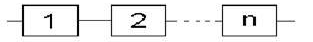
\includegraphics[width=.5\linewidth]{assets/connect}
	  \caption{CCН основного соединения}
	  \label{img:20-0}
	\end{figure}

	При условии независимости отказов элементов в системе (поток отказов без последствий) ВБР системы с основным соединением будет равна произведению ВБР её элементов:
	\begin{equation}
		P_{sys}(t) = \prod\limits_{i = 1}^{n}P_{i}(t).
	\end{equation}

	Если интенсивность отказов не постоянна, тогда:
	\begin{gather}
		P_{sys}(t) = e^{-\sum\limits_{i = 1}^{n}\;\int\limits_{0}^{t}\lambda_{i}(\tau)d\tau};\\
		T_{1,sys} = \int\limits_{0}^{\infty}P_{sys}(t)dt.
	\end{gather}

	Если интенсивность отказов постоянна, тогда:
	\begin{gather}
		P_{sys}(t) = e^{-\sum\limits_{i = 1}^{n}\lambda_{i}t};\\
		T_{1,sys} = \int\limits_{0}^{\infty}P_{sys}(t)dt;\\
		f_{sys}(t) = -\frac{d P_{sys}(t)}{d t} = \sum\limits_{i = 1}^{n}\lambda_{i}e^{-\sum\limits_{i = 1}^{n}\lambda_{i}t};\\
		\lambda_{sys} = \frac{P_{sys}(t)}{f_{sys}(t)} = \sum\limits_{i = 1}^{n}\lambda_{i}.
	\end{gather}

	Основные свойства системы с основным соединением элементов без восстановления: 
	\begin{enumerate}
		\item C увеличением количества элементов системы надёжность системы уменьшается; 
		\item Надёжность системы в целом заведомо ниже надёжности любого элемента системы;
		\item Устойчивость экспоненциального закона надёжности.
	\end{enumerate}


	\section{Размерное квантование}
Квантоворазмерный эффект (квантовый размерный эффект) — изменение термодинамических и кинетических свойств кристалла, когда хотя бы один из его геометрических размеров становится соизмеримым с длиной волны де Бройля электронов. Этот эффект связан с квантованием энергии носителей заряда, движение которых ограничено в одном, двух или трёх направлениях.\\

Волны де Бройля — волны вероятности, определяющие плотность вероятности обнаружения объекта в заданной точке конфигурационного пространства. В соответствии с принятой терминологией говорят, что волны де Бройля связаны с любыми частицами и отражают их волновую природу.

\begin{gather} 
	\lambda = \frac{h}{p} = \frac{h}{\hbar k} = \frac{h}{mv};\\
	\psi(x, t) = A*e^{\frac{i}{\hbar}(px-Et)} = A*e^{i(kx-\omega t)}.
\end{gather}

В зависимости от размерности пространства электронный газ имеет различный закон дисперсии, плотность состояний и эффективную плотность состояний, см табл.~\ref{tab:gE} \cite{Harrison}.

\begin{center}
    \begin{longtable}{| c | c | c | c |}
	    \caption{Плотность состояний и эффективная плотность состояний для низкоразмерных систем}
	    \label{tab:gE}
	    \\ \hline
	    Размерность & Закон дисперсии & $g(E)$ & $G(E)$ \\
	    \hline \endfirsthead
	    \subcaption{Продолжение таблицы~\ref{tab:gE}}
	    \\ \hline \endhead
	    \hline \subcaption{Продолжение на след. стр.}
	    \endfoot
	    \hline \endlastfoot
	    3D, bulk & $\frac{\hbar^{2}}{2m}(k_{x}^{2}+k_{y}^{2}+k_{z}^{2})$ & $ \frac{2^{\frac{1}{2}}m^{\frac{3}{2}}}{\pi^{2}\hbar^{3}}E^{\frac{1}{2}} $ & $\frac{(2m)^{\frac{3}{2}}}{3\pi^{2}\hbar^{3}}E^{\frac{3}{2}}$\\
	    \hline
	    2D, well & $\frac{\hbar^{2}}{2m}(k_{x}^{2}+k_{y}^{2})+\frac{\pi^{2}\hbar^{2}n^{2}}{2mL^{2}}$ & $\frac{m}{\pi\hbar^{2}}$ & $\frac{m}{\pi\hbar^{2}}E$\\
	    \hline
	    1D, wire & $\frac{\hbar^{2}}{2m}(k_{x}^{2}) + \frac{\pi^{2}\hbar^{2}}{2m}\Big( \frac{n_{1}^{2}}{L_{1}^{2}} + \frac{n_{2}^{2}}{L_{2}^{2}} \Big)$ & $\frac{\sqrt{m}}{\sqrt{2}\pi\hbar}E^{-\frac{1}{2}}$ & $\frac{\sqrt{2m}}{\pi\hbar}E^{\frac{1}{2}}$\\
	    \hline
	    0D, dot & $\frac{\pi^{2}\hbar^{2}}{2m}\Big( \frac{n_{1}^{2}}{L_{1}^{2}} + \frac{n_{2}^{2}}{L_{2}^{2}} + \frac{n_{3}^{2}}{L_{3}^{2}} \Big)$ & $2\delta E$ & $2$
    \end{longtable}
\end{center}

% \begin{figure}[h]
% 	\centering
% 	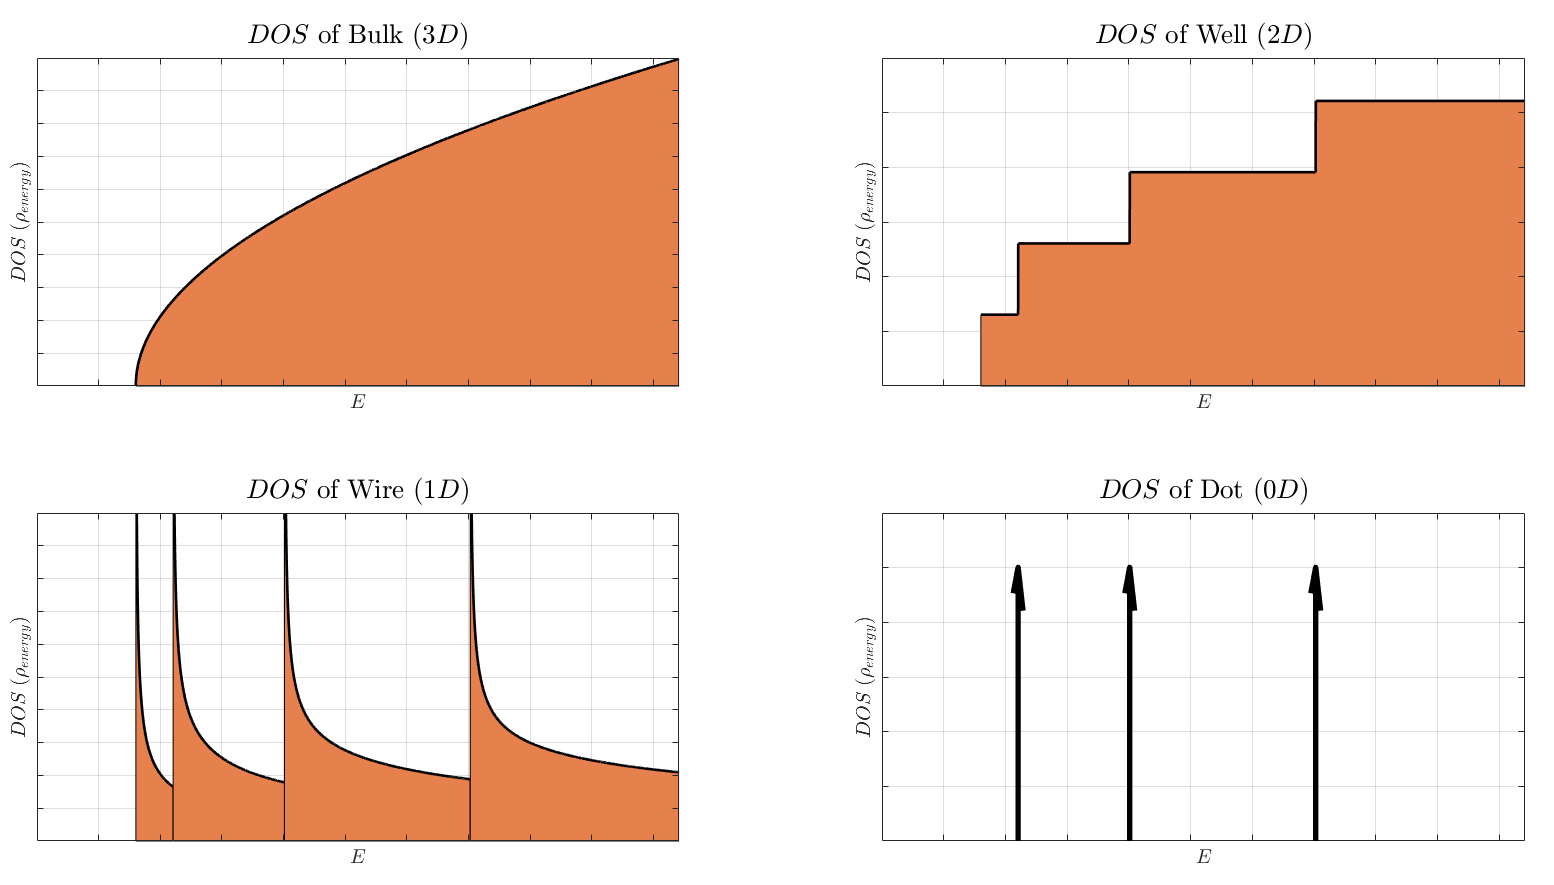
\includegraphics[width=\textwidth]{gE.png}
% 	\caption{Плотность состояний в 3D, 2D, 1D, 0D, где $g(E) = \rho_{energy}$}
% 	\label{DOS}
% \end{figure}

\subsection{Трехмерное тело}
Рассмотрим 3D кристалл (bulk) на рис.~\ref{fig:3DBulk}:\\

\noindent
\begin{minipage}[b]{0.4\textwidth}
	\centering
    \includegraphics[width=\textwidth]{assets/3DBulk}
\end{minipage}
\hfill
\begin{minipage}[b]{0.55\textwidth}
	\centering
	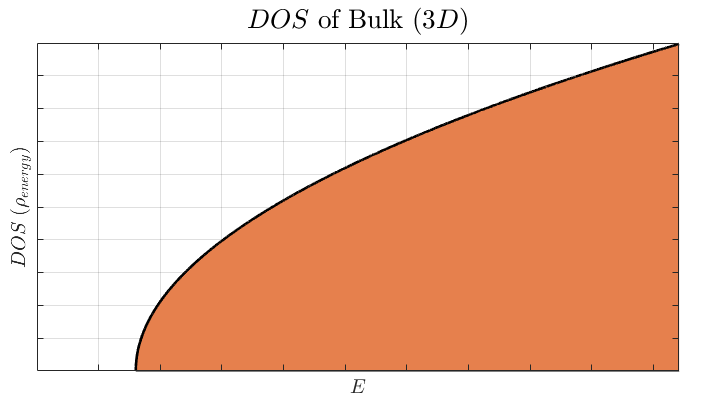
\includegraphics[width=\textwidth]{assets/gE3D}
\end{minipage}

\begin{figure}[h]
	\centering
	% \includegraphics[scale=0.5]{3DBulk.png}
	\caption{k-пространство (шар)}
	\label{fig:3DBulk}
\end{figure}

Число состояний частицы $G(E)$ и плотность состояний $g(E)$, энергия которых не превышает некоторого фиксированного значения $E$, находятся из формул:
\begin{gather*} 
	G(E) = \frac{V_{sphere}}{V_{single-state}} = J_{z}\frac{\frac{1}{8}\frac{4}{3}\pi k^{3}}{\frac{\pi^3}{V}} = \frac{k^{3}V}{3\pi^{2}} = \frac{(2m)^{\frac{3}{2}}V}{3\pi^{2}\hbar^{3}}E^{\frac{3}{2}};\\
	k = \frac{\sqrt{2mE}}{\hbar};\\
	g(E) = \frac{dG(E)}{dE} = \frac{(2E)^{\frac{1}{2}}m^{\frac{3}{2}}}{\pi^{2}\hbar^{3}}V.
\end{gather*}

\subsection{Двухмерное тело}
Рассмотрим 2D кристалл (well) на рис.~\ref{fig:2DWire}.
\begin{gather*} 
	G(E) = \frac{V_{circul}}{V_{single-state}} = J_{z}\frac{\frac{1}{4}\pi k^{2}}{\frac{\pi^2}{S}} = \frac{k^{2}}{2\pi} = \frac{mS}{\pi\hbar^{2}}E;\\
	g(E) = \frac{dG(E)}{dE} = \frac{m}{\pi\hbar^{2}}S.
\end{gather*}

\noindent
\begin{minipage}[b]{0.35\textwidth}
	\centering
    \includegraphics[width=\textwidth]{assets/2DWire}
\end{minipage}
\hfill
\begin{minipage}[b]{0.6\textwidth}
	\centering
	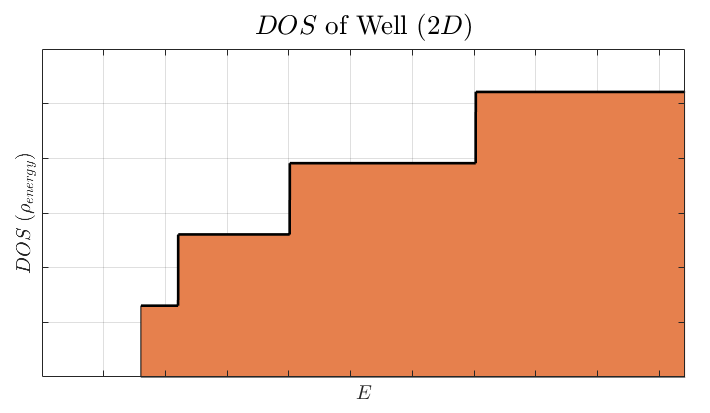
\includegraphics[width=\textwidth]{assets/gE2D}
\end{minipage}

\begin{figure}[h]
	\centering
	% \includegraphics[scale=0.5]{2DWire.png}
	\caption{k-пространство (круг)}
	\label{fig:2DWire}
\end{figure}

\subsection{Одномерное тело}
Рассмотрим 1D кристалл (wire)  на рис.~\ref{fig:1Ddot}:

\noindent
\begin{minipage}[b]{0.3\textwidth}
	\centering
    \includegraphics[width=\textwidth]{assets/1Ddot}
\end{minipage}
\hfill
\begin{minipage}[b]{0.6\textwidth}
	\centering
	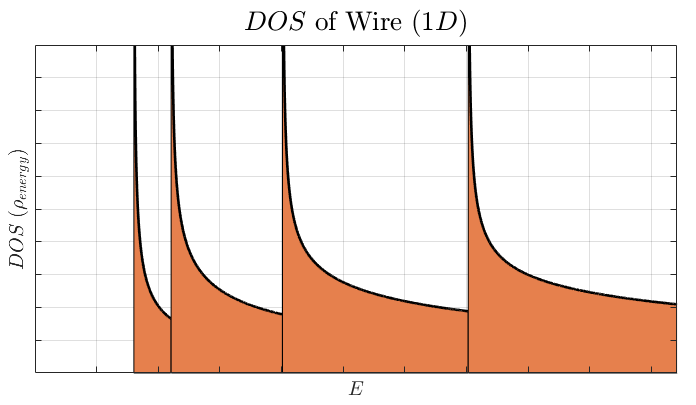
\includegraphics[width=\textwidth]{assets/gE1D}
\end{minipage}

\begin{figure}[h]
	\centering
	% \includegraphics[scale=0.5]{1Ddot.png}
	\caption{k-пространство (линия)}
	\label{fig:1Ddot}
\end{figure}

\begin{gather*} 
	G(E) = \frac{V_{line}}{V_{single-state}} = J_{z}\frac{k}{\frac{\pi}{L}} = \frac{kL}{pi} = \frac{\sqrt{2m}L}{\pi\hbar}E^{\frac{1}{2}};\\
	g(E) = \frac{dG(E)}{dE} = \frac{\sqrt{m}L}{\sqrt{2}\pi\hbar}E^{-\frac{1}{2}}.
\end{gather*}

$J_{z}$ -- определяет число состояний не связанных с перемещением частицы в пространстве (например, число возможных проекций спина). В нашем случае, для электрона $J_{z}=2$.
	\section{Деградация}
Деградация~--- процесс ухудшения характеристик какого-либо объекта или явления с течением времени, постепенное ухудшение, упадок, снижение качества.

Изучая деградацию ГС рассматривают следующие параметры:
\begin{itemize}
	\item Вольт-амперная характеристика (ВАХ);
	\item Высота потенциального барьера (ПБ);
	\item Ширина потенциального барьера;
	\item Ширина потенциальной ямы (ПЯ);
	\item Т.п...
\end{itemize}

Все параметры ГС тесно связаны с друг с другом. Изменение одного влечет изменение остальных.

Один из примеров ГС~--- это резонансно-туннельный диод (РТД). РТД используют в качестве преобразователя частот в смесителях, где преобразование частот зависит от формы ВАХ РТД, которая подвержена деградации.

Форма ВАХ задается ГС активной области РТД. Исследование и моделирование деградации ВАХ ГС важная задача. В зависимости от отрасли необходимо гарантировать различную $T_{\gamma=0.999}$.

Одна из причин деградации ВАХ ГС~--- диффузионное размытие профиля дна зоны проводимости ($E_{c}$).

\section{Диффузия}
Диффузия — это обусловленный хаотическим тепловым движением перенос атомов, он может стать направленным под действием градиента концентрации или температуры.

Диффундировать могут как собственные атомы решетки, так и атомы растворенных в полупроводнике элементов, а также точечные дефекты структуры кристалла — междоузельные атомы и вакансии.

\subsection{Законы Фика}
\begin{definition}{\textsc{Первый закон Фика}}
	Плотность потока вещества пропорциональна коэффициенту диффузии ($D$) и градиенту концентрации ($C$). Является стационарным уравнением.
	\begin{gather}
		\overline{J} = - D \nabla C;\\
		\overline{J}_{x} = - \overline{e}_{x}D_{x} \frac{\delta}{\delta x} C_{x}.\\
	\end{gather}
\end{definition}

\begin{definition}{\textsc{Второй закон Фика}}
	Связывает пространственное и временное изменения концентрации.
 	\begin{gather}
		\frac{\delta}{\delta t}C = - \nabla (D \nabla C);\\
		\frac{\delta}{\delta t}C_{x} = - \frac{\delta}{\delta x} D_{x} \frac{\delta}{\delta x} C_{x}.
	\end{gather}
\end{definition}

\subsection{Механизмы диффузии примесей}

Вакансионный механизм диффузии — заключается в миграции атомов по кристаллической решётке при помощи вакансий.

Межузельный механизм диффузии — заключается в переносе вещества межузельными атомами.

Прямой обмен атомов местами — заключается в том, что два соседних атома одним прыжком обмениваются местами в решетке кристалла.

\subsection{Коэффициент диффузии}
Коэффициент диффузии в терминах случайных блужданий можно записать(для простой кубической решетки):
\begin{equation}
	D = \frac{1}{6}\lambda^{2}\nu,
\end{equation}
\begin{conditions}
	$\lambda$ & расстояние между соседними кристаллографическими плоскостями;\\
	$\nu$ & частота скачков диффундирующих атомов.
\end{conditions}

Частота скачков $\nu$ зависит от температуры ($T$)
\begin{equation}
	\nu = \nu_{0}\exp\bigg[-\frac{E_{a}}{k_{B}T}\bigg],
\end{equation}
\begin{conditions}
	$E_{a}$ & энергия активации;\\
	$k_{B}$ & константа Больцмана;\\
	$T$ & температура атома;\\
	$\mu_{0}$ & константа.
\end{conditions}

Коэффициент диффузии ($D$)~--- макроскопическая величина, которая определяется экспериментально. Коэффициент диффузии зависит от температуры(T) по закону Аррениуса:
\begin{equation}
	D = D_{0}\exp\bigg[-\frac{E_{a}}{k_{B}T}\bigg],
\end{equation}
\begin{conditions}
	$D_{0}$ & предэкспоненциальный множитель.
\end{conditions}

Коэффициент ($D_{0}$) и энергия активации ($E_{a}$) не зависят от температуры.

\subsection{Коэффициент диффузии $Al$, $Si$ в $GaAs$}
Основным механизмом диффузии $Al$ и $Si$ в $GaAs$ является диффузия по вакансиям галлия ($V_{Ga}$). Это связано с тем, что атомы $Al$ и $Si$ имеют сходные массы и размеры. 

С учетом эффекта уровня Ферми получено в работах ~\cite{getMeshkov}, ~\cite{Meshkov}, ~\cite{Meshkov}, ~\cite{Makeev} получено соотношение коэффициента диффузии $Al$ и $Si$ в $GaAs$:
\begin{equation}
	D_{Al,Si} = D_{i-GaAs}\Big( \frac{n}{n_{i}} \Big)^{3} = D_{0}\exp\bigg[-\frac{3.5}{k_{B}T}\bigg]\Big( \frac{n}{n_{i}} \Big)^{3},
\end{equation}
\begin{conditions}
	$n$ & концентрация электронов в зоне проводимости;\\
	$n_{i}$ & концентрация собственных носителей заряда.
\end{conditions}
	\section{Деградация приборов на основе гетероструктур}
Деградация~--- процесс ухудшения характеристик какого-либо объекта c течением времени.

% Изучая деградацию ГС рассматривают следующие параметры:
% \begin{itemize}
	%\item Вольт-амперная характеристика (ВАХ);
% 	\item Высота потенциального барьера (ПБ);
%	\item Ширина потенциального барьера;
%	\item Ширина потенциальной ямы (ПЯ);
%	\item Т.д...
%\end{itemize}

Деградация параметров гетероструктуры во времени связана с диффузионным размытие ГП и ГС в целом. Зонная структура ГС определяет режим работы, а зонная структура ГС зависит от химического состава, поэтому диффузионное размытие изменяет зонную диаграмму и режимы работы прибора на основе ГС.
% ГС используют для построения резонансно-туннельный диод (РТД), квантовых точек (КТ), транзисторов с высокой подвижностью электронов (HEMT) и так далее. 

 % Химический состав ГС определяет ее зонную структуру, из чего вытекают особенности работы тех или иных устройств на ГС.

Факторы влияющие на диффузионное размытие: 
\begin{itemize}
	\item Градиент температуры; 
	\item Градиент концентрации; 
	\item Градиент давления;
	\item Наличие деффектов;
	\item и т.д... 
\end{itemize}

Диффузионное размытие под действием градиента концентрации описывается с помощью законов Фика.

\section{Диффузия}
Диффузия — это обусловленный хаотическим тепловым движением перенос атомов, он может стать направленным под действием градиента концентрации или температуры.

Диффундировать могут как собственные атомы решетки, так и атомы растворенных в полупроводнике элементов, а также точечные дефекты структуры кристалла — междоузельные атомы и вакансии.

\subsection{Законы Фика}
Первый закон Фика говорит, что плотность потока вещества пропорциональна коэффициенту диффузии ($D$) и градиенту концентрации ($C$). Является стационарным уравнением.
\begin{gather}
	\overline{J} = - D \nabla C;\\
	\overline{J}_{x} = - \overline{e}_{x}D_{x} \frac{\delta}{\delta x} C_{x}.\\
\end{gather}

Второй закон Фика связывает пространственное и временное изменения концентрации.
\begin{gather}
	\frac{\delta}{\delta t}C = - \nabla (D \nabla C);\\
	\frac{\delta}{\delta t}C_{x} = - \frac{\delta}{\delta x} D_{x} \frac{\delta}{\delta x} C_{x}.
\end{gather}

\subsection{Механизмы диффузии}

Вакансионный механизм диффузии — заключается в миграции атомов по кристаллической решётке при помощи вакансий.

Межузельный механизм диффузии — заключается в переносе вещества межузельными атомами.

Прямой обмен атомов местами — заключается в том, что два соседних атома одним прыжком обмениваются местами в решетке кристалла.

\subsection{Коэффициент диффузии}
% Коэффициент диффузии в терминах случайных блужданий можно записать(для простой кубической решетки):
% \begin{equation}
% 	D = \frac{1}{6}\lambda^{2}\nu,
% \end{equation}
% \begin{conditions}
% 	$\lambda$ & расстояние между соседними кристаллографическими плоскостями;\\
% 	$\nu$ & частота скачков диффундирующих атомов.
% \end{conditions}

% Частота скачков $\nu$ зависит от температуры ($T$)
% \begin{equation}
% 	\nu = \nu_{0}\exp\bigg[-\frac{E_{a}}{k_{B}T}\bigg],
% \end{equation}
% \begin{conditions}
% 	$E_{a}$ & энергия активации;\\
% 	$k_{B}$ & константа Больцмана;\\
% 	$T$ & температура атома;\\
% 	$\mu_{0}$ & константа.
% \end{conditions}

Коэффициент диффузии ($D$)~--- макроскопическая величина, которая определяется экспериментально. Коэффициент диффузии зависит от температуры ($T$) по закону Аррениуса:
\begin{equation}
	\label{eq:DConst}
	D = D_{0}\exp\bigg[-\frac{E_{a}}{k_{B}T}\bigg],
\end{equation}
\begin{conditions}
	$D_{0}$ & предэкспоненциальный множитель.
\end{conditions}
Коэффициент ($D_{0}$) и энергия активации ($E_{a}$) не зависят от температуры.

% \subsection{Коэффициент диффузии $Al$, $Si$ в $GaAs$}
Основным механизмом диффузии $Al$ и $Si$ в $GaAs$ является диффузия по вакансиям галлия ($V_{Ga}$). Это связано с тем, что атомы $Al$ и $Si$ имеют сходные массы и размеры. 

С учетом эффекта уровня Ферми коэффициент диффузии $Al$ и $Si$ в $GaAs$ получен в работах ~\cite{getMeshkov}, ~\cite{Makeev}, ~\cite{Gosele}:
\begin{equation}
	\label{eq:DNd}
	D_{Al,Si} = D_{i-GaAs}\Big( \frac{N_{D}}{n_{i}} \Big)^{3} = D_{0}\exp\bigg[-\frac{3.5}{k_{B}T}\bigg]\Big( \frac{n}{n_{i}} \Big)^{3},
\end{equation}
\begin{conditions}
	$n$ & концентрация донорной примеси ($Si$);\\
	$n_{i}$ & концентрация собственных носителей заряда.
\end{conditions}

Концентрация собственных носителей заряда:
\begin{gather}
	n_{i} = \sqrt{N_{c}N_{v}}\exp\!\bigg[ - \frac{E_{g}}{2k_{B}T} \bigg];\\
	N_{c} = 2\Big[ \frac{2\pi m_{e}^{\ast}k_{B}T}{h^{2}} \Big]^{\frac{3}{2}};\\
	N_{v} = 2\Big[ \frac{2\pi m_{h}^{\ast}k_{B}T}{h^{2}} \Big]^{\frac{3}{2}},
\end{gather}
\begin{conditions}
	$E_{g}$ & ширина запрещенной зоны (ЗЗ) п/п.
\end{conditions}
	\section{Плотность тока через ГС}
Один из способов расчета плотности тока через гетероструктуру~--- это формула Цу--Есаки:
\begin{equation}
	\label{eq:J}
	J(V) = \frac{2mek_{B}T}{(2\pi)^{2}\hbar^{3}}\int\limits_{0}^{\infty}T(E)D(E)dE,
\end{equation}
\begin{conditions}
	$J(V)$ & плотность тока при приложенном напряжении $V$;\\
	$T(E)$ & прозрачность гетероструктуры;\\
	$D(E)$ & функция снабжения электронами;\\
	$m$ & эффективная масса электрона;\\
	$e$ & заряд электрона;\\
	$T$ & температура;\\
	$\hbar$ & постоянная Дирака;\\
	$k_{B}$ & постоянная Больцмана.
\end{conditions}
\begin{equation}
	\label{eq:De}
	D(E) = \ln\frac{1 + \exp{\frac{E_{F}-E}{k_{B}T}} }{ 1 + \exp{\frac{E_{F}-E-eV}{k_{B}T}} },
\end{equation}
\begin{conditions}
	\label{eq:D}
	$E_{F}$ & уровень Ферми;\\
	$V$ & приложенное напряжение.
\end{conditions}

Коэффициент прозрачности гетероструктуры определяется   как   отношение потока вероятности прошедших  через  структуру электронов  в  правом резервуаре к  падающим  на  неё  электронам  в  левом  резервуаре.  Поток вероятности находится из формулы:
\begin{equation}
	\label{eq:jP}
	\overline{j} = \frac{i\hbar}{2m}(\psi\nabla\psi^{*} - \psi^{*}\nabla\psi),
\end{equation}
\begin{conditions}
	$\psi$ & волновая функция электрона.
\end{conditions}
Будем рассматривать электроны, приходящие из левого контакта. Левому контакту соответствуют волновые функции $\psi_{L}$, а в правому~---  $\psi_{R}$.
\begin{gather}
	\label{eq:psiL}
	\psi_{L} = \exp [ik_{L}z];\\
	\label{eq:psiR}
	\psi_{R} = T_{L}\psi_{L} = T_{L}\exp [ik_{L}z],
\end{gather}
\begin{conditions}
	$T_{L}$ & Амплитуда прошедшей волновой функции;\\
	$k_{L}$ & волновой вектор в левом резервуаре.
\end{conditions}
Тогда коэффициент туннельной прозрачности:
\begin{equation}
	\label{eq:T}
	T(E) = |T_{L}|^{2}\frac{|k_{R}|m_{L}}{|k_{L}|m_{R}},
\end{equation}
\begin{conditions}
	$k_{R}$ & волновой вектор в правом резервуаре;\\
	$m_{R}$ & эффективная масса электрона в правом резервуаре;\\
	$m_{L}$ & эффективная масса электрона в левом резервуаре.
\end{conditions}
\subsection{Уравнение Шредингера}
Для нахождения волновых функций необходимо решить уравнение Шредингера. Для твердого тела уравнение Шредингера имеет вид:
\begin{gather*}
	-\frac{\hbar}{2}\Bigg[ \bigg( \frac{1}{m}\sum\limits_{i}\Delta_{i} + \sum\limits_{i}\frac{\Delta_{i}}{M_{i}} \bigg) + \frac{1}{2}\sum\limits_{i, j\neq i}\frac{e^{2}}{k_{k}|\overline{r_{i}} - \overline{r_{j}}|} + \frac{1}{2}\sum\limits_{i, j\neq i}\frac{Z_{i}Z_{j}e^{2}}{k_{k}|\overline{R_{i}} - \overline{R_{j}}|} -\\ - \frac{1}{2}\sum\limits_{i, j\neq i}\frac{Z_{i}e^{2}}{k_{k}|\overline{R_{i}} - \overline{r_{j}}|} \Bigg]\psi = E\psi
\end{gather*}
\begin{conditions}
	$M_{i}$ & масса атомного остова;\\
	$k_{k}$ & постоянная Кулона;\\
	$Z $& атомное число;\\
	$\frac{\Delta_{i}}{m}$ & кинетическая энергия $i$-ого электрона;\\
	$\frac{\Delta_{i}}{M_{i}}$ & кинетическая энергия $i$-ого атомного остова;\\
	$\frac{e^{2}}{k_{k}|\overline{r_{i}} - \overline{r_{j}}|}$ & потенциальное взаимодействие $i$ и $j$ электрона;\\
	$\frac{Z_{i}Z_{j}e^{2}}{k_{k}|\overline{R_{i}} - \overline{R_{j}}|}$ & потенциальное взаимодействие остовов;\\
	$\frac{Z_{i}e^{2}}{k_{k}|\overline{R_{i}} - \overline{r_{j}}|}$ & потенциальное взаимодействие остова и электрона.
\end{conditions}

Ряд приближений упрощает полное уравнение Шредингера для твердого тела:
\begin{enumerate}
	\item Атомные остовы находятся в состоянии покоя;
	\item Электрон движется, не взаимодействуя с другими электронами, в некотором эффективном поле, создаваемым остальными электронами;
	\item Движение электрона в периодическом потенциале заменяется на эффективную массу.
\end{enumerate}
Упрощенное уравнение Шредингера:
\begin{equation}
	\label{eq:ShredGen}
	-\frac{\hbar^{2}}{2m}\Delta\psi + U\psi = E\psi,
\end{equation}
\begin{conditions}
	$ U $ & потенциальный профиль.
\end{conditions}
Одномерное ур. Шредингера:
\begin{equation}
	\label{eq:Shred}
	-\frac{\hbar^{2}}{2m}\frac{d^{2}}{dz^{2}}\psi(z) + U(z)\psi(z) = E\psi(z).
\end{equation}
Для решения уравнения на границе гетероперехода рассматриваются условия непрерывности волновой функции и непрерывности потока плотности вероятности~--- эти условия так же называются условием Бастарда:
\begin{equation}
	\label{eq:Bastard}
	\begin{cases}
		\psi_{I} = \psi_{II};\\
		\frac{1}{m_{I}}\frac{d}{dz}\psi_{I} = \frac{1}{m_{II}}\frac{d}{dz}\psi_{II},
	\end{cases}
\end{equation}
\begin{conditions}
	$m_{I}$& эффективная масса в $I$ структуре;\\
	$m_{II}$& эффективная масса во $II$ структуре;\\
	$\psi_{I}$& волновая функция в $I$ структуре;\\
	$\psi_{II}$& волновая функция во $II$ структуре.
\end{conditions}
Учтем эффективную массу в ур.~\ref{eq:Shred}:
\begin{equation}
	\label{eq:ShredM}
	-\frac{\hbar^{2}}{2}\frac{d}{dz}\frac{1}{m(z)}\frac{d}{dz}\psi(z) + U(z)\psi(z) = E\psi(z).
\end{equation}
В случае произвольного потенциального рельефа для решения уравнения Шредингера применяются численные методы.

\subsection{Учёт распределения заряда}
Приближение Хартри сводит многоэлектронное уравнение Шредингера к одноэлектронному, в котором электрон движется в некотором эффективном поле, создаваемом другими электронами. Это поле называется самосогласованным.
Распределение заряда в структуре определяется с помощью уравнения Пуассона:
\begin{equation}
	\label{eq:poisson}
	\frac{d}{dz}\varepsilon(z)\frac{d}{z}V_{s} = \frac{e}{\varepsilon_{0}}[n(z) - N_{D}(z)],
\end{equation}
\begin{conditions}
	$\varepsilon$ & относительная электрическая проницаемость;\\
	$\varepsilon_{0}$ & диэлектрическая постоянная;\\
	$V_{s}$ & самосогласованный потенциал;\\
	$e$ & заряд электрона;\\
	$n$ & концентрация электронов;\\
	$N_{D}$ & концентрация донорной примеси.
\end{conditions}

В приконтактных областях концентрация электронов ($n_{L}$, $n_{R}$) находится с помощью (\ref{eq:n}). Приконтактные области высоколегированны и уровень Ферми лежит выше дна ЗП. Положение уровня Ферми можно найти с помощью (\ref{eq:EFn+}) или как корень уравнения (\ref{eq:n}).

Нахождение концентрации электронов в активной области производится с учетом плотности вероятности волновых функций \cite{Moskaluk}:
\begin{equation}
	\label{eq:n2D}
	n = \iiint\limits_{-\infty}^{+\infty}|\psi(\overline{k})|^{2}N(\overline{k})d\overline{k} = \iiint\limits_{-\infty}^{+\infty}|\psi(\overline{k})|^{2}g_{3D}(\overline{k})f(\overline{k})d\overline{k},
\end{equation}
\begin{conditions}
	$N(\overline{k})$ & количество разрешенных состояний;\\
	$g_{3D}$ & плотность состояний в $3D$;\\
	$f(\overline{k})$ & .
\end{conditions}

Энергия электронов:
\begin{equation}
	E(\overline{k}) = E_{x} + E_{y} + E_{z} = \frac{\hbar k_{x}^{2}}{2m} + \frac{\hbar k_{y}^{2}}{2m} + \frac{\hbar k_{z}^{2}}{2m} - eV;
\end{equation}
\begin{conditions}
	$k_{i}$ & волновой вектор в направлении $i$;\\
	$V$ & приложенное напряжение.
\end{conditions}

Так как волновую функцию $\psi(x, y,z )$ можно представить в виде:
\begin{equation}
	\psi(x, y, z) = \psi(x)\psi(y)\psi(z),
\end{equation}
а концентрацию электронов в активной области $n$ разделить на попадающие из левого и правого резервуаров:
\begin{gather}
	n = n_{L} + n_{R};\\
	\label{eq:nPsi}
	n_{L(R)} = \frac{2^{1/2}m^{3/2}k_{B}T}{(2\pi)^{2}\hbar^{3}}\int\limits_{U_{l(r)}}^{\infty} \frac{|\psi_{L(R)}|^{2}}{\sqrt{E - U_{L(R)}}} \ln \bigg( 1 + \exp\bigg[ -\frac{E - E_{F} - U_{la(ra)}}{k_{B}T} \bigg] \bigg),
\end{gather}
\begin{conditions}
	$U_{l(r)}$ & потенциал на границе приконтактной и активной области;\\
	$U_{la(ra)}$ & потенциал на границе активной области.
\end{conditions}
Формулу (\ref{eq:nPsi}) можно интерпретировать, как произведение локальной плотности состояний в активной области $g^{*}_{L(R)}(E)$ на распределение электронов по энергии ($f_{L(R)}(E)$):
\begin{gather}
	g^{*}_{L(R)}(E) = \frac{2^{1/2}m^{3/2}k_{B}T}{(2\pi)^{2}\hbar^{3}}|\psi_{L(R)}|^{2};\\
	f_{L(R)}(E) =  \frac{1}{\sqrt{E - U_{la(ra)}}} \ln \bigg( 1 + \exp\bigg[ -\frac{E - E_{F} - U_{L(R)}}{k_{B}T} \bigg] \bigg).
\end{gather}

Таким образом, чтобы найти распределение электронов в активной области~--- необходимо решить систему Шредингера-Пуассона.
\begin{equation}
	\label{eq:P-S}
	\begin{cases}
		\frac{d}{dz}\varepsilon(z)\frac{d}{z}V_{s} = \frac{e}{\varepsilon_{0}}[n(z) - N_{D}(z)];\\
		-\frac{\hbar^{2}}{2}\frac{d}{dz}\frac{1}{m(z)}\frac{d}{dz}\psi(z) + U(z)\psi(z) = E\psi(z);
	\end{cases}
\end{equation}

	\section{Метод конечных разностей для расчета токоперенос через ГС}
	\section{Влияние пространственного заряда}
	\section{Решение уравение Шредингера-Пуассона}

% \chapter{Исследовательская часть}
	\chapter{Математический аппарат для моделирования}

\section{Метод конечных разностей}
Суть метода конечных разностей заключается в аппроксимации дифференциальных операторов отношением конечных разностей. Так например производную некоторой функции $y(x)$ в точке $x_{0}$ ($\dot{y}(x_{0})$) можно представить \cite{Samarski}:
\begin{gather}
	\dot{y}_{+}(x_{0}) = \frac{d}{dx}y(x_{0}) = \frac{y(x_{0} + \Delta x) - y(x_{0})}{\Delta x };\\
	\dot{y}_{-}(x_{0}) = \frac{d}{dx}y(x_{0}) = \frac{ y(x_{0}) - y(x_{0} - \Delta x)}{\Delta x };\\
	\dot{y}_{-}(x_{0}) = \dot{y}_{+}(x_{0}) = \frac{d}{dx}y(x_{0}),
\end{gather}
\begin{conditions}
	$\dot{y}_{-}$ & производная слева;\\
	$\dot{y}_{+}$ & производная справа;\\
	$\Delta x$ & приращение аргумента (шаг сетки).
\end{conditions}

$\Delta x$ -- это шаг нашей конечно-разностной схемы (аппроксимации). Если шаг сетки постоянен, то говорят о регулярной сетке, иначе о нерегулярной. Мы будем рассматривать только регулярные сетки. Далее вместо $\Delta x$ будет использовать $\Delta$.

Из выше сказанного можно найти трехточечную аппроксимацию второй производной $y(x)$:
\begin{gather}
	\frac{d^{2}}{dx^{2}}y(x_{0}) = \frac{\dot{y}_{+} - \dot{y}_{-}}{\Delta} = \frac{y(x_{0} + \Delta) - 2y(x_{0}) + y(x_{0} - \Delta)}{ \Delta^{2}}.
\end{gather}

Для связи конечно-разностной схемы по времени и координате для нестационарного уравнения диффузии (\ref{eq:F2}) воспользуемся двухточечной апроксимацией первой производной по времени и трехточечной апроксимацие второй производной по координате: 
\begin{equation}
	\label{eq:xt}
	\frac{C^{j+1}_{i} - C^{j}_{i}}{\Delta t} = \frac{C^{j}_{i-1} - 2C^{j}_{i} + C^{j}_{i+1}}{\Delta^{2}},
\end{equation}

\begin{conditions}
	$C^{j}_{i}$ & значение функции в точке $i$, в момент времени $j$;\\
	$\Delta t$ & шаг сетки по времени;\\
	$\Delta x$ & шаг сетки по координате.
\end{conditions}

% Конечно разностную схему (\ref{eq:xt}) наглядно можно представить так:
% \begin{figure}
% 	\centering
% 	\includegraphics[width=0.9\linewidth]{assets/Diffusion}
% 	\caption{Графическая схема для конечно-разностной схемы (\ref{eq:xt})}
% 	\label{fig:xt}
% \end{figure}
% \begin{conditions}
% 	$S(x, t)$ & состояние системы в момент $t$ и точке $x$;\\
% 	$\Delta x$ & приращение по координате;\\
% 	$\Delta t$ & приращение по времени.
% \end{conditions}

	\section{Метод конечных разностей для решения одномерного нестационарного уравнения диффузии}
\subsection{Коэффициент диффузии не зависит от концентрации}
% Одномерное нестационарное уравнение диффузии, соответствующее второму закону Фика имеет вид:
% \begin{equation}\label{eq:difft}
% 	\frac{\delta}{\delta t} C = D\frac{\delta^{2}}{\delta x^2} C;
% \end{equation}

% Аппроксимация первой производной по времени в момент времени $t_{i}$ концентрации $C_{j}(t_{i}) = C^{i}_{j}$ в точке $j$:
% \begin{equation}\label{eq:diffdt1}
% 	\frac{\delta}{\delta t} C^{i}_{j} = \frac{C^{i+1}_{j} - C^{i}_{j}}{\Delta t};
% \end{equation}

% Аппроксимация первой производной по координате в момент времени $t_{i}$ концентрации $C_{j}(t_{i}) = C^{i}_{j}$ в точке $j$:
% \begin{equation}\label{eq:diffdx1}
% 	J^{i}_{j} = \frac{\delta}{\delta x} C^{i}_{j} = \frac{C^{i}_{j+1} - C^{i}_{j}}{\Delta x};
% \end{equation}

% Аппроксимация второй производной по координате в момент времени $t_{i}$ концентрации $C_{j}(t_{i}) = C^{i}_{j}$ в точке $j$:
% \begin{equation*}
% 	\frac{\delta^{2}}{\delta x^{2}} C^{i}_{j} = \frac{\delta}{\delta x}\bigg[ \frac{C^{i}_{j+1} - C^{i}_{j}}{\Delta x} \bigg] = \frac{ \frac{C^{i}_{j+1} - C^{i}_{j}}{\Delta x} - \frac{C^{i}_{j} - C^{i}_{j-1}}{\Delta x}}{\Delta x} = 
% \end{equation*}
% \begin{equation}\label{eq:diffdx2}
% 	= \frac{C^{i}_{j+1} - 2C^{i}_{j} + C^{i}_{j-1}}{\Delta x^2};
% \end{equation}

% Подставляя в (\ref{eq:difft}) аппроксимацию производных (\ref{eq:diffdt1}), (\ref{eq:diffdx2}), получим связь $C^{i+1}_{j}$ с $C^{i}_{j}$, т.е. изменение концентрации через $\Delta t$:

% \begin{equation}\label{eq:diffFD}
% 	C^{i+1}_{j} = \lambda C^{i}_{j-1} + (1 - 2\lambda)C^{i}_{j} + \lambda C^{i}_{j+1},
% \end{equation}
% где $\lambda = \frac{D\Delta t}{\Delta x^2}$~---  связь коэффициента диффузии и шагов по сетке времени и координаты.

% Уравнение (\ref{eq:diffFD}) справедливо для всех не крайних точек конечно разностной схемы, при коэффициенте диффузии не зависящем от концентрации.

% Выделим два граничных приближения для концентрации:
% \begin{enumerate}
% 	\item <<Закрытая система>> ~--- концентрация на границе не изменяется ($J_{0}^{i} = 0$, $J_{N+1}^{i} = 0$);
% 	\item <<Открытая система>> ~--- поток частиц подходящий к границе равен потоку уходящих частиц ($J_{0}^{i} = J_{1}^{i}$, $J_{N}^{i} = J_{N+1}^{i}$).
% \end{enumerate}

% \begin{figure}
%     \centering
%     \begin{subfigure}[b]{0.45\textwidth}
%         \includegraphics[width=\textwidth]{CD}
%         \caption{A gull}
%         \label{fig:gull}
%     \end{subfigure}
%     \begin{subfigure}[b]{0.45\textwidth}
%         \includegraphics[width=\textwidth]{OD}
%         \caption{A mouse}
%         \label{fig:mouse}
%     \end{subfigure}
%     \caption{Pictures of animals}\label{fig:animals}
% \end{figure}

% \noindent
% \begin{minipage}{0.4\textwidth}
% 	\centering
% 	\includegraphics[width=\linewidth]{assets/CD}
% 	а)
% \end{minipage}
% ~
% \begin{minipage}{0.6\textwidth}
% 	\centering
% 	\includegraphics[width=\linewidth]{assets/OD}
% 	б)
% \end{minipage}
% \begin{figure}
% 	\centering
% 	% \includegraphics[width=0.9\linewidth]{assets/CD}
% 	\caption{a) <<Закрытая>>, б) <<Открытая>> система диффузии}
% 	\label{fig:DS}
% \end{figure}



% \begin{figure}
% 	\centering
% 	\includegraphics[width=0.8\linewidth]{assets/OD}
% 	\caption{"Открытая" система диффузии}
% 	\label{fig:OD}
% \end{figure}


<<Закрытая система>> ~--- концентрация на границе не изменяется ($J_{0}^{i} = 0$, $J_{N+1}^{i} = 0$):
\begin{equation}
	\begin{cases}
		C^{i+1}_{1} = (1 - \lambda)C^{i}_{1} + \lambda C^{i}_{2};\\
		C^{i+1}_{j} = \lambda C^{i}_{j-1} + (1 - 2\lambda)C^{i}_{j} + \lambda C^{i}_{j+1},\,j \in [2,\,\dots,\,N-1];\\
		C^{i+1}_{N} = (1 - \lambda)C^{i}_{N} + \lambda C^{i}_{N-1};\\
		\lambda = D\frac{\Delta t}{\Delta x^{2}}.
	\end{cases}
\end{equation}

<<Открытая система>> ~--- поток частиц подходящий к границе равен потоку уходящих частиц ($J_{0}^{i} = J_{1}^{i}$, $J_{N}^{i} = J_{N+1}^{i}$):
\begin{equation}
	\label{eq:DDiffConst}
	\begin{cases}
		C^{i+1}_{1} = C^{i}_{1};\\
		C^{i+1}_{j} = \lambda C^{i}_{j-1} + (1 - 2\lambda)C^{i}_{j} + \lambda C^{i}_{j+1},\,j \in [2,\,\dots,\,N-1];\\
		C^{i+1}_{N} = C^{i}_{N};\\
		\lambda = D\frac{\Delta t}{\Delta x^{2}}.
	\end{cases}
\end{equation}

\subsection{Коэффициент диффузии зависит от концентрации}

% Если коэффициенте диффузии (D) зависит от концентрации, тогда уравнение диффузии принимает вид:

% \begin{equation}\label{eq:diffD(x)t}
% 	\frac{\delta}{\delta t} C = \frac{\delta}{\delta x}D\frac{\delta}{\delta x} C;
% \end{equation}

Проводя рассуждения аналогичные предыдущему параграфу получит конечно-разностную схему для открытой схемы:
\begin{equation}
	\begin{cases}
		C^{i+1}_{1} = C^{i}_{1};\\
		C^{i+1}_{j} = \lambda_{-}^{i} C^{i}_{j-1} + (1 - \lambda^{i}_{+} - \lambda^{i}_{-})C^{i}_{j} + \lambda^{i}_{+} C^{i}_{j+1},\,j \in [2,\,\dots,\,N-1];\\
		C^{i+1}_{N} = C^{i}_{N};\\
		\lambda^{i}_{+} = D_{j+}^{i}\frac{\Delta t}{\Delta x^{2}};\\
		\lambda^{i}_{-} = D_{j-}^{i}\frac{\Delta t}{\Delta x^{2}}.
	\end{cases}
\end{equation}

	% \section{Моделирование токопереноса через ГС}
% \subsection{Алгоритм моделирования токопереноса через ГС}
% \begin{figure}[h]
%   \centering
%   \includegraphics[width=0.7\linewidth]{assets/AlgJ}
%   \caption{Блок схема алгорит моделирования токопереноса через ГС}
%   \label{img:AlgJ}
% \end{figure}

% \subsection{Результат моделирования}
% \begin{figure}[h]
%   \centering
%   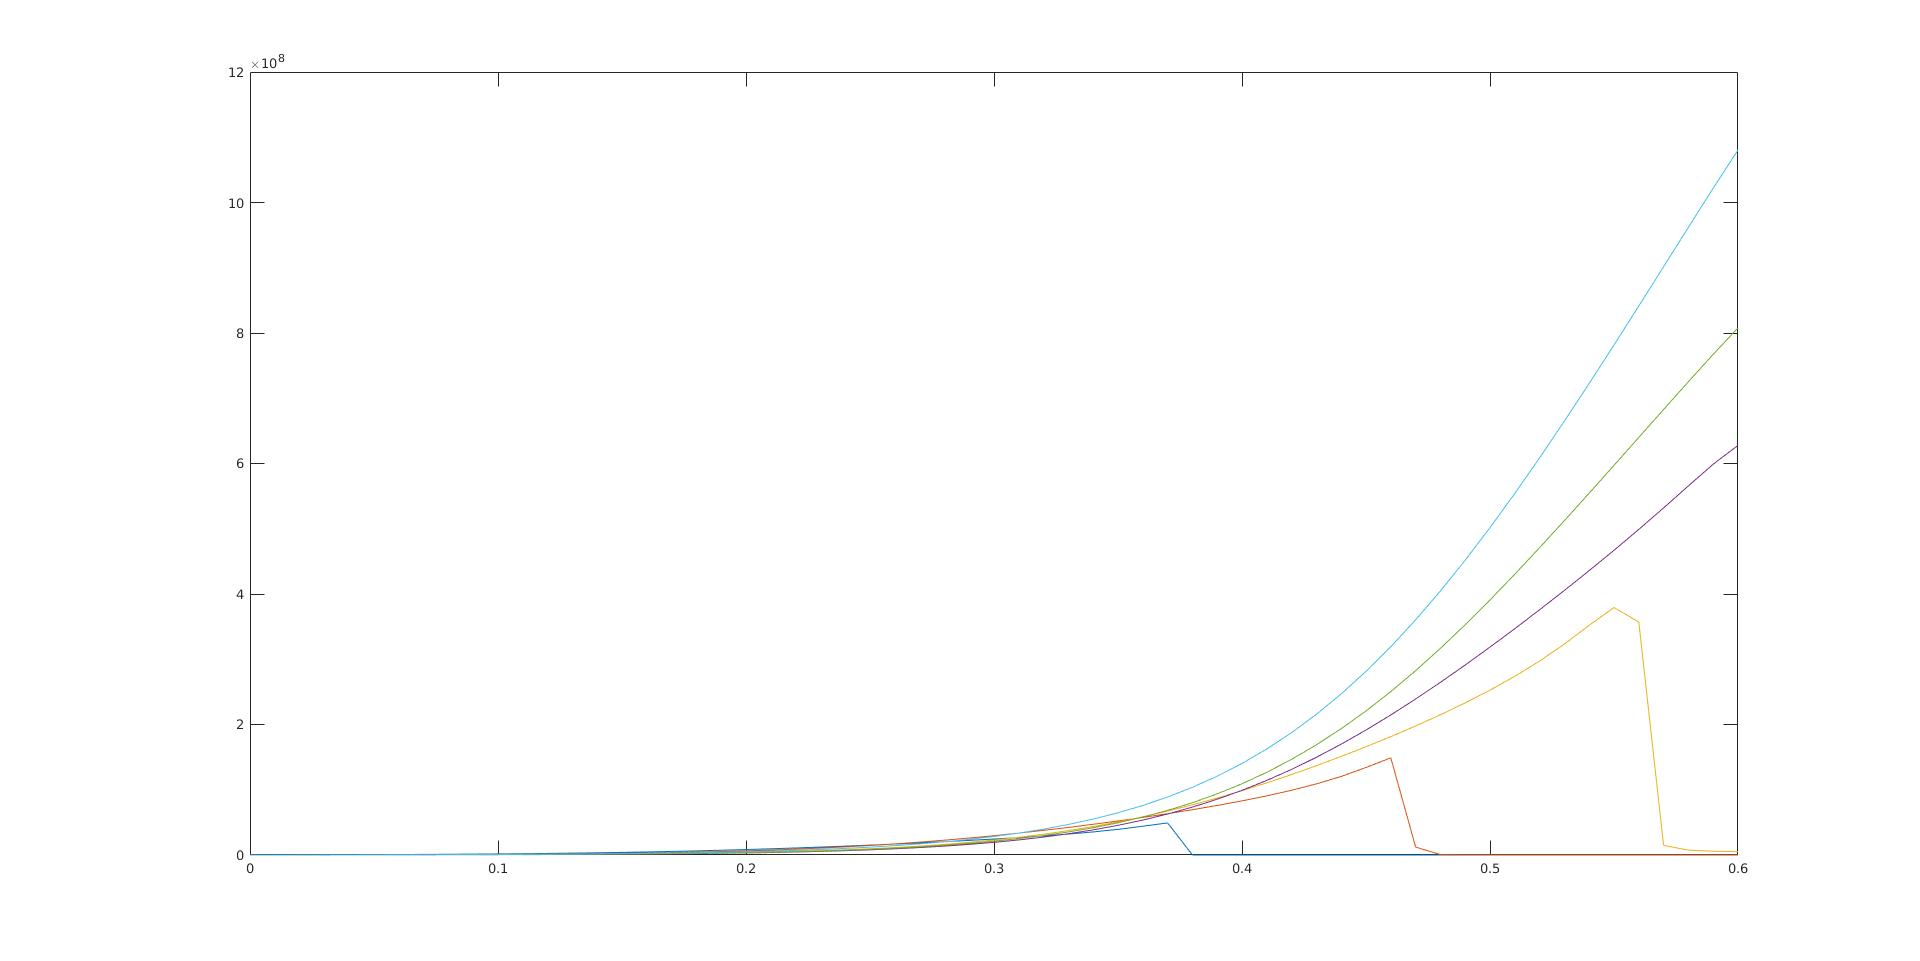
\includegraphics[width=1.1\linewidth]{assets/degrI25}
%   \caption{Результат моделирования токопереноса через гетероструктуру}
%   \label{img:degrI25}
% \end{figure}

\section{Моделирование диффузионного размытия $n^{+}\!-\!GaAs/i\!-\!GaAs/i\!-\!Al_{45}Ga_{55}As/ n^{+}\!-\!GaAs$}

\begin{figure}[h]
  \centering
  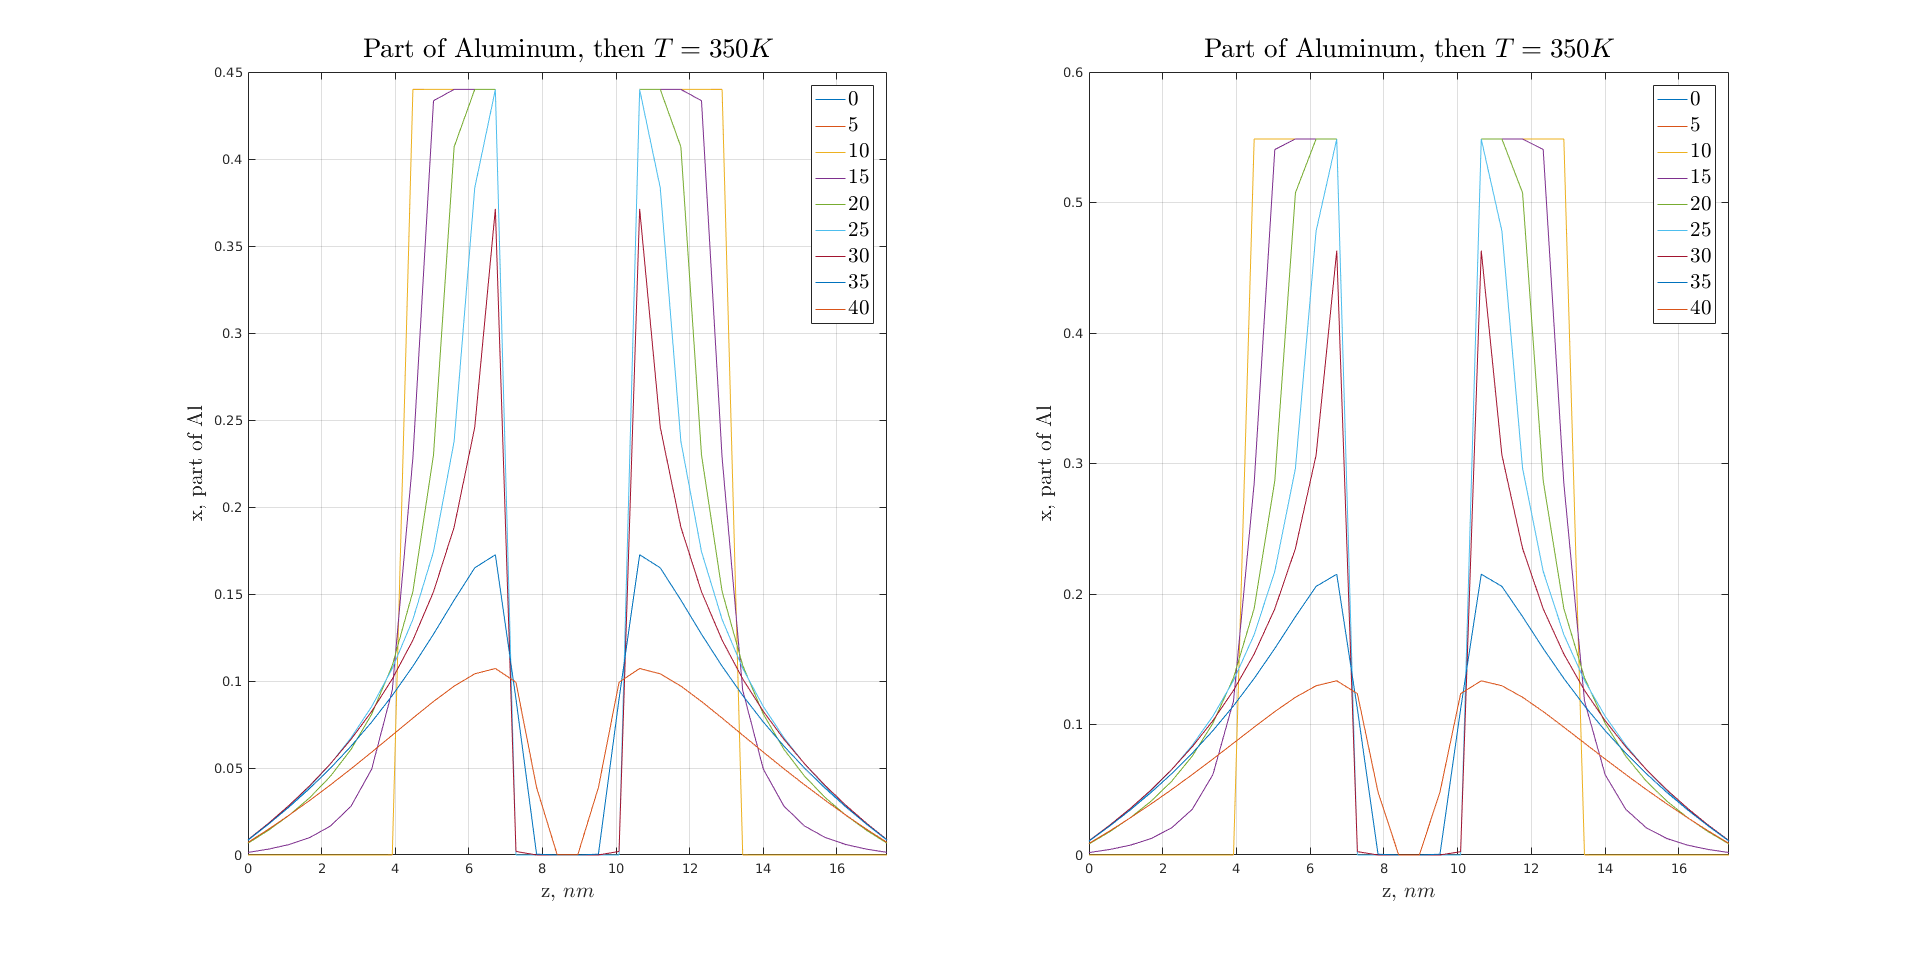
\includegraphics[width=0.9\linewidth]{DAlGaAs_Si}
  \caption{Диффузионное размытие}
\end{figure}

\begin{figure}[h]
  \centering
  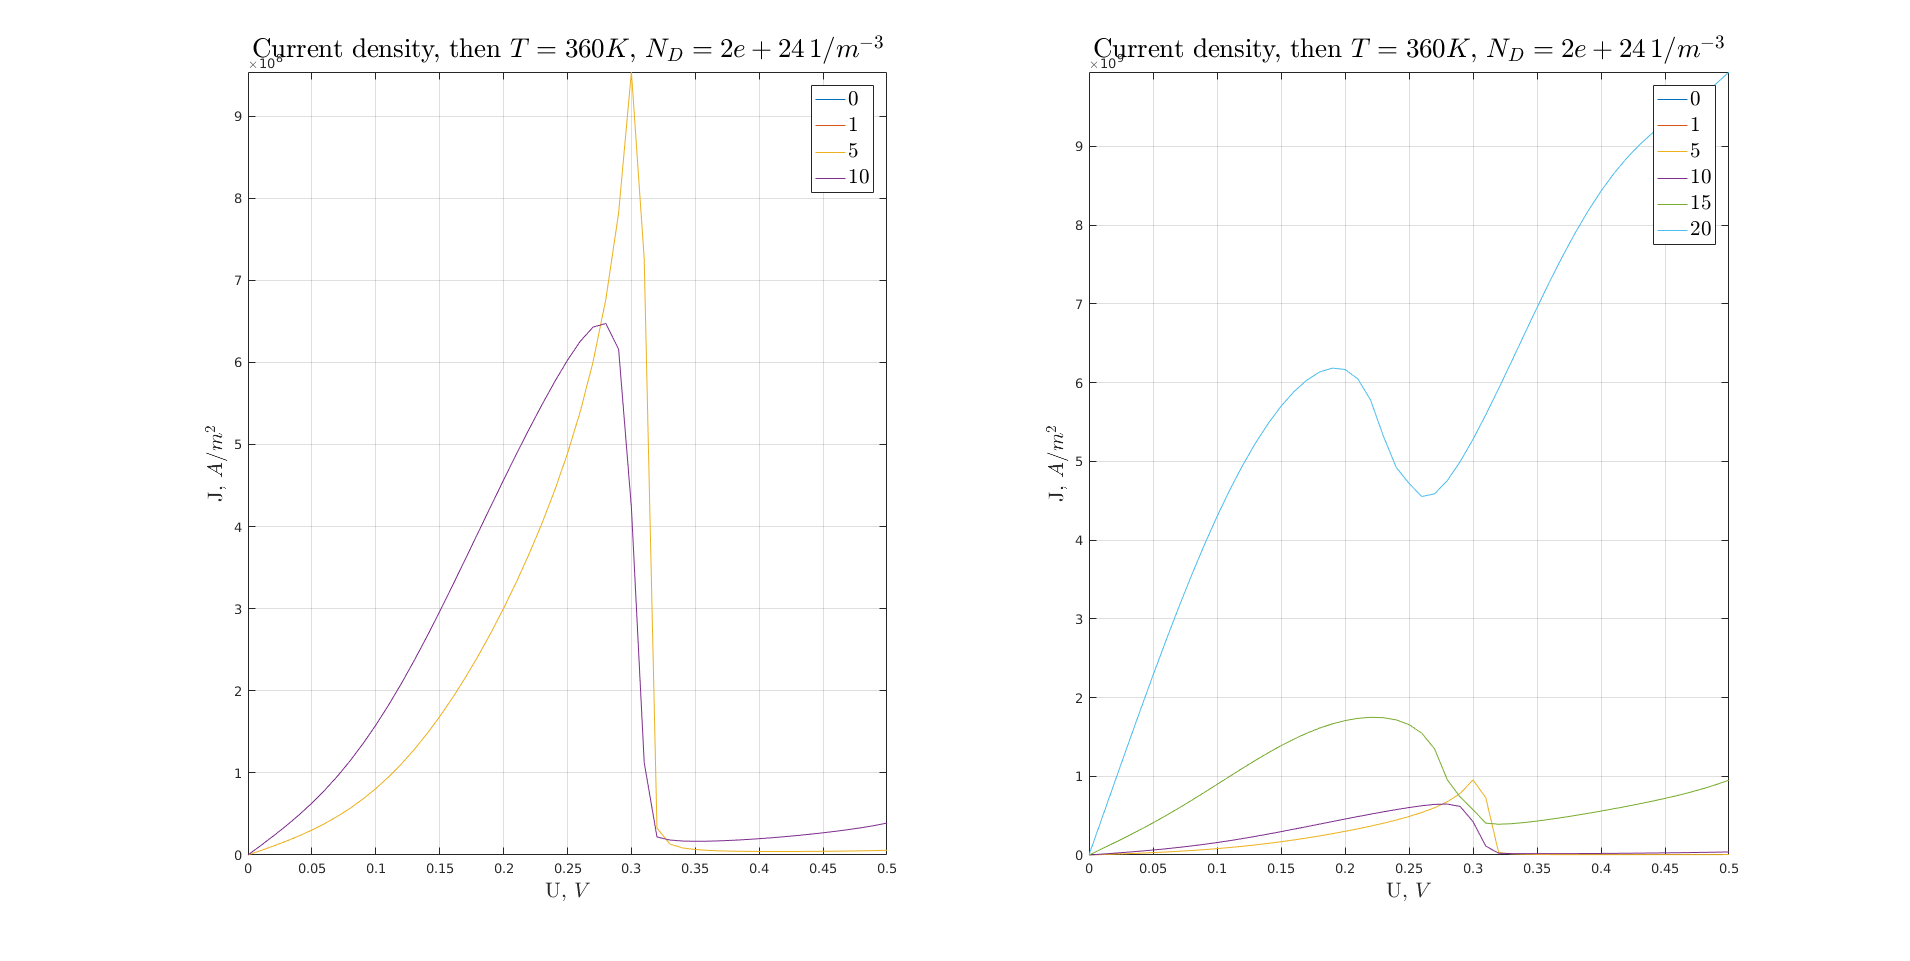
\includegraphics[width=0.9\linewidth]{JDAlGaAs_Si}
  \caption{Деградация ВАХ}
\end{figure}

\begin{figure}[h]
  \centering
  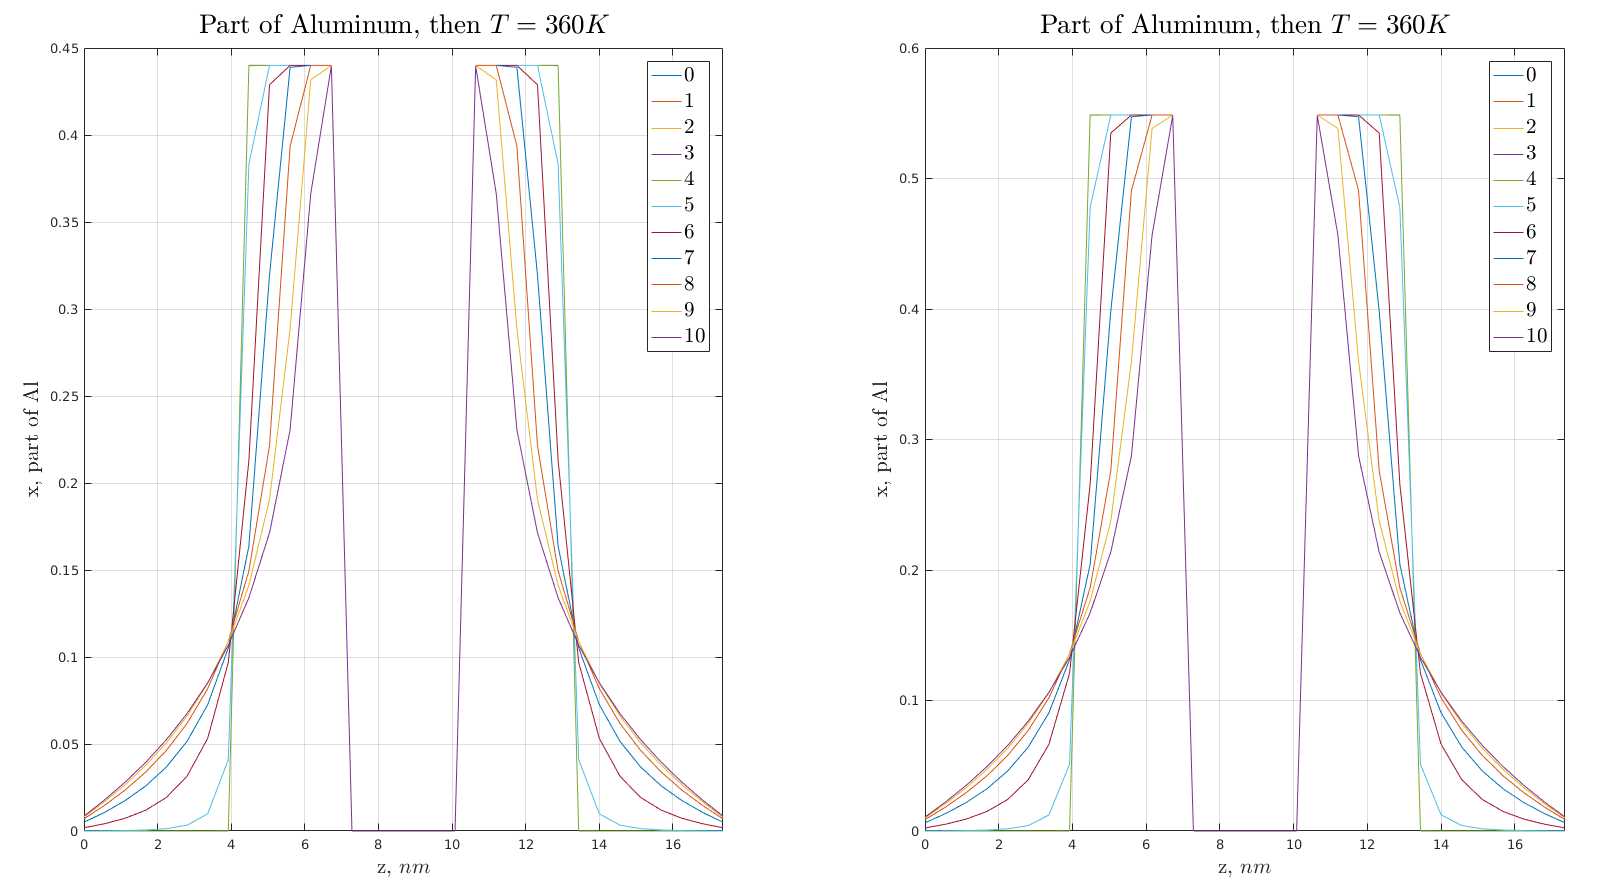
\includegraphics[width=\linewidth]{DAlGaAs_Si_360}
  \caption{Диффузионное размытие при повышении температуры}
\end{figure}

\begin{figure}[h]
  \centering
  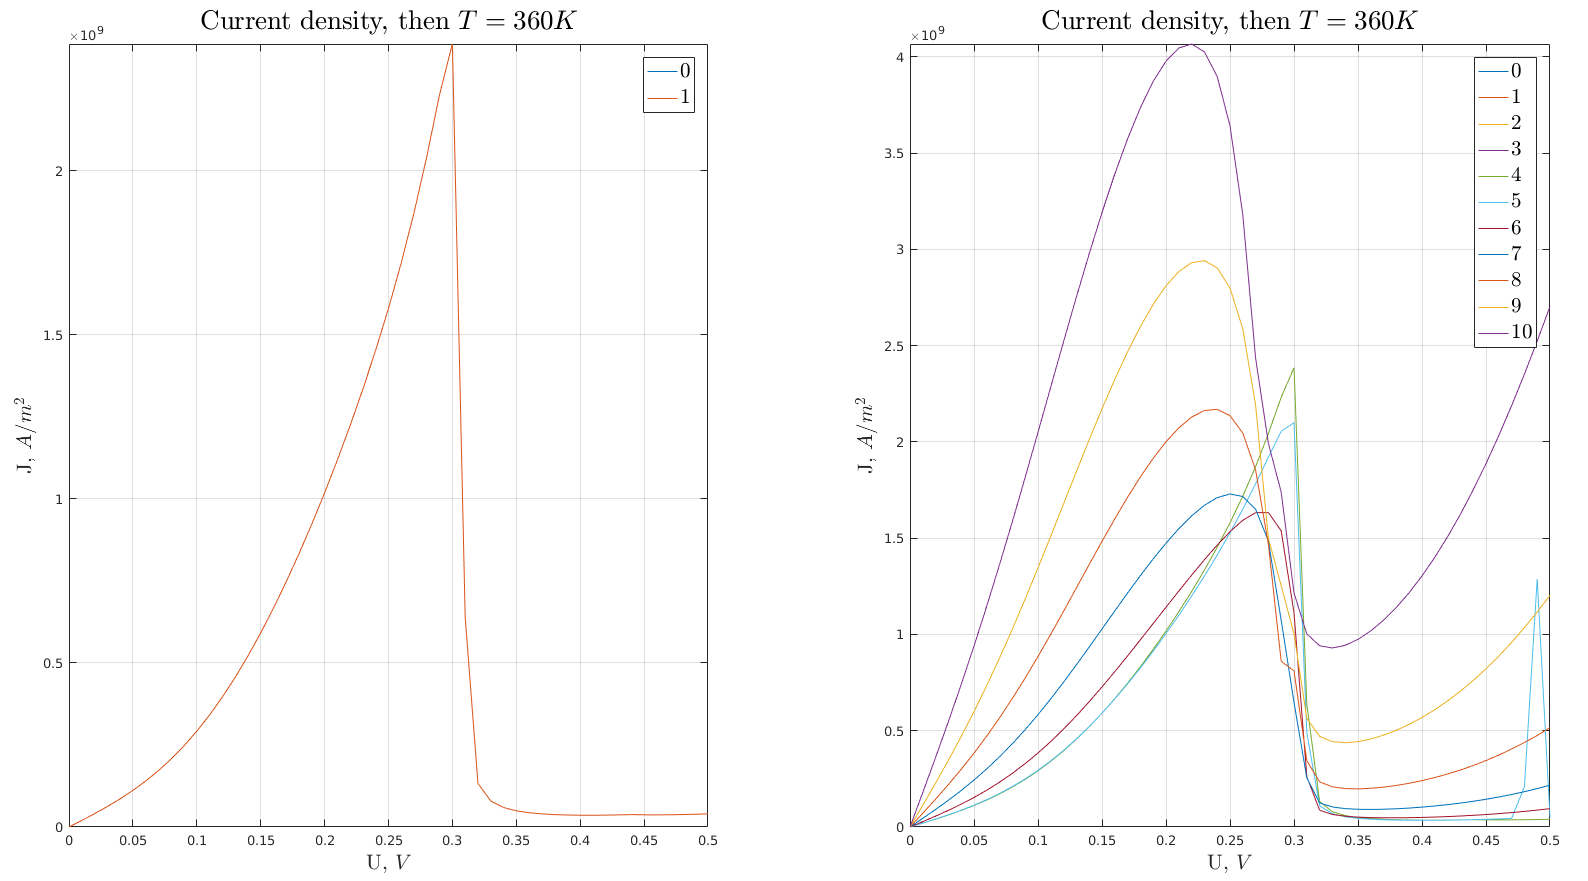
\includegraphics[width=\linewidth]{JDAlGaAs_Si_360}
  \caption{Деградация ВАХ при повышении температуры}
\end{figure}
% \chapter{Моделирование}
	\chapter{Исследование параметров РТГС на основе $Al_{x}Ga_{1-x}As$}
\section{Исследование параметров ямы}
Энергетический спектр в бесконечно глубокой потенциальной яме:
\begin{gather}
	\label{eq:En}
	E_{n} = \frac{\pi^{2}\hbar^{2}n^{2}}{2mL^{2}};\\
	\Delta E_{n} = E_{n+1} - E_{n} = \frac{\pi^{2}\hbar^{2}}{2mL^{2}}(2n + 1);\\
	\label{eq:dEn1}
	\Delta E_{1} = \min(\Delta E_{n}) = \frac{3\pi^{2}\hbar^{2}}{2mL^{2}},
\end{gather}
\begin{conditions}
	$E_{n}$ & энергия $n$-ого связного состояния;\\
	$\hbar$ & постоянная Дирака;\\
	$n$ & номер ($1,\,,2,\dots$) связного состояния;\\
	$L$ & ширина ямы.
\end{conditions}

Из зависимостей~\ref{eq:En},~\ref{eq:dEn1}  видно, что с увеличением ширины ямы, энергия основного состояния уменьшается ($n = 1$), так же, как и минимальное расстояние, между энергетическими уровнями. Условие размерного квантования для потенциальной ямы:
\begin{equation}
	\Delta E_{1} \gg 3k_{B}T.
\end{equation}

В случаи ямы с конечной высотой, энергия основного и остальных состояний понижается, при этом минимальная высота барьера ограничивает состояние с максимальной энергией. В потенциальной яме конечной высоты всегда будет хотя бы одно связное состояние.

\subsection{Исследование глубины ямы}
Варьирую процентное содержание $Al$ в $Al_{x}Ga_{1-x}As$, можно изменять высоту барьеров и глубину ямы соответственно. Рассмотрим вольт-амперную характеристику и прозрачность резонансно-туннельной структуры.

Так как в ходе деградации ГС высота барьеров будет уменьшаться, так как атомы $Al$ будут диффундировать в структуру из барьеров, рассмотрим РГТС (рис.~\ref{img:rtgs}) с высотой потенциальных барьеров:
\begin{enumerate}
	\item $1.0 eV$;
	\item $0.7 eV$;
	\item $0.5 eV$;
	\item $0.3 eV$.
\end{enumerate}

\subsubsection{Прозрачность РТГС}
\begin{figure}[h]
	\centering
	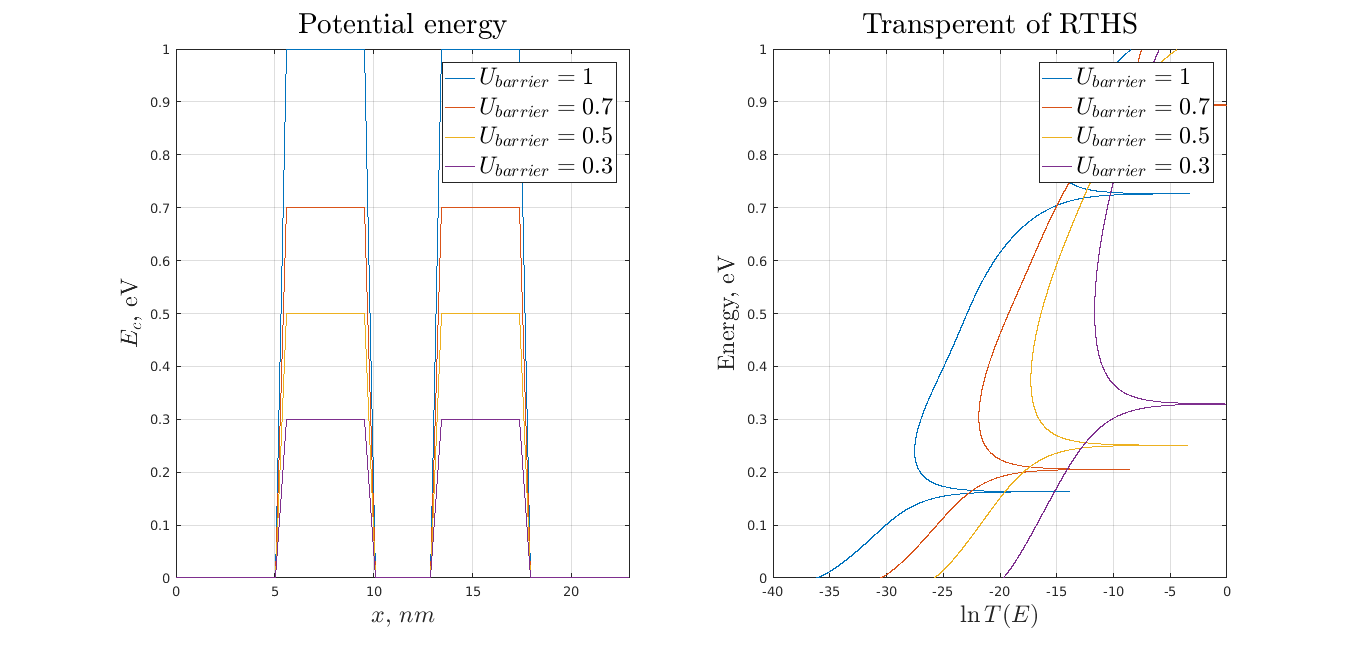
\includegraphics[scale=0.5]{qwt.png}
	\caption{Прозрачность РТГС при различных высотах потенциального барьера}
	\label{fig:qwt}
\end{figure}

\subsubsection{ВАХ РТГС}
\begin{figure}[h]
	\centering
	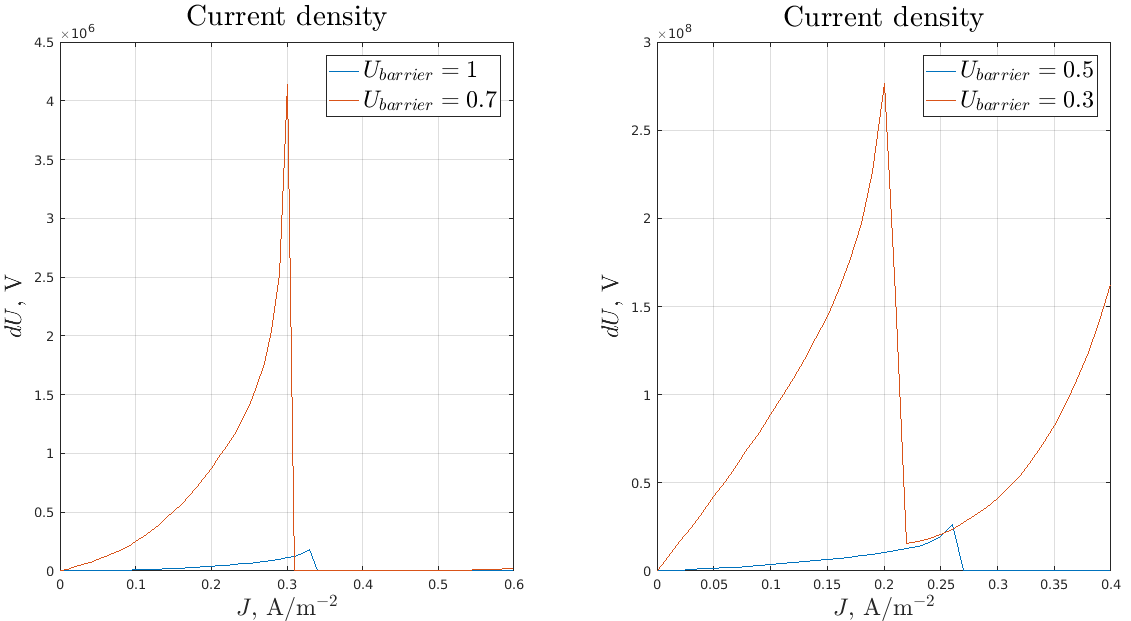
\includegraphics[scale=0.5]{qwj.png}
	\caption{Плотность тока через РТГС при различных высотах потенциального барьера}
	\label{fig:qwj}
\end{figure}

\subsection{Исследование ширины ямы}
Уменьшая или увеличивая количество монослоев, мы варьируем ширину ямы в РТГС. Для примера рассмотрим РТГС:
\begin{enumerate}
	\item $10$ монослоев;
	\item $7$ монослоев;
	\item $5$ монослоев;
	\item $3$ монослоев.
\end{enumerate}
\subsubsection{Прозрачность РТГС}
\begin{figure}[h]
	\centering
	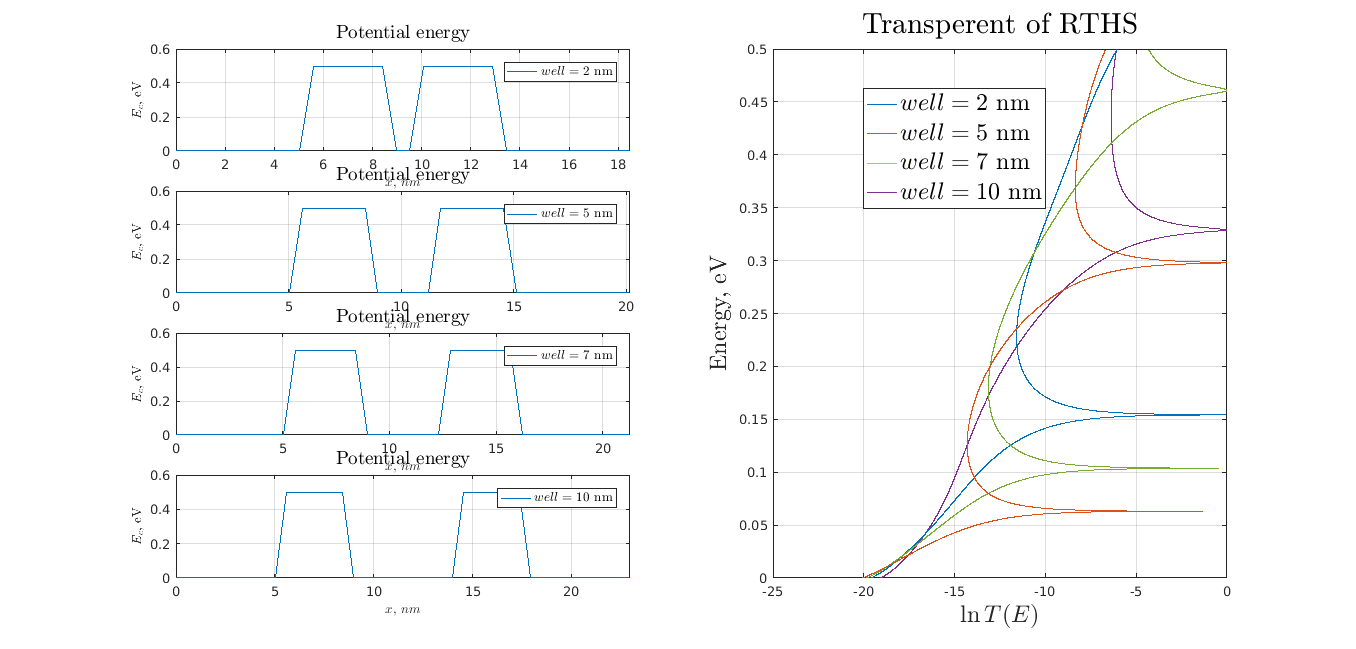
\includegraphics[scale=0.5]{qwwt.png}
	\caption{Прозрачность РТГС при различных ширинах потенциальной ямы}
	\label{fig:qwwt}
\end{figure}
\subsubsection{ВАХ РТГС}
\begin{figure}[h]
	\centering
	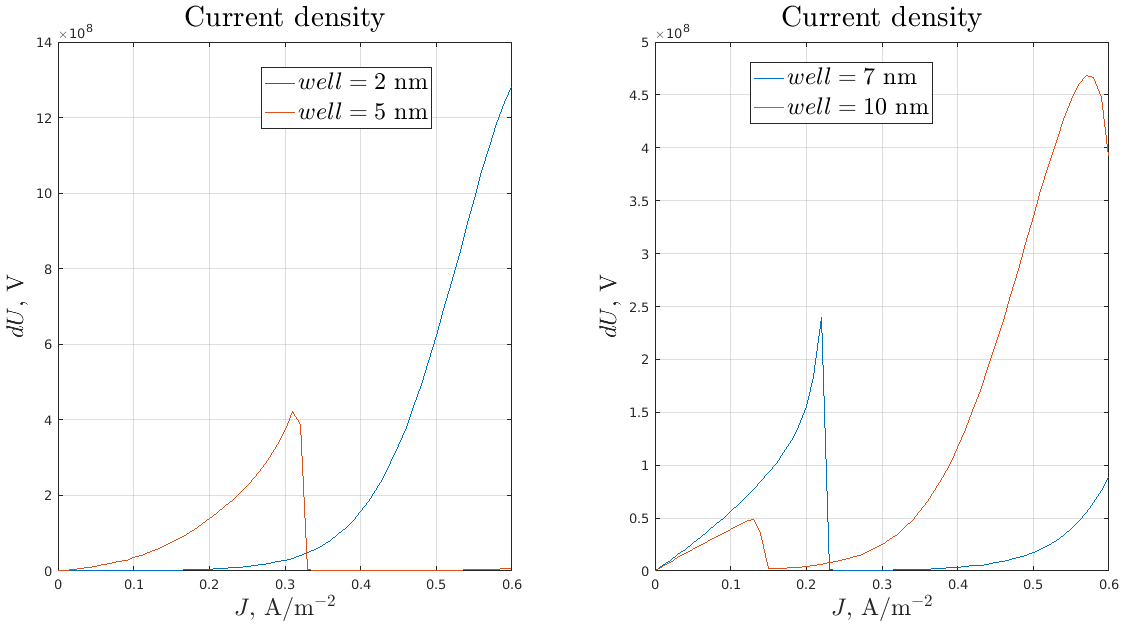
\includegraphics[scale=0.5]{qwwj.png}
	\caption{Плотность тока через РТГС при различных ширинах потенциальной ямы}
	\label{fig:qwwj}
\end{figure}
	% \section{Моделирование старения ГС}
% \subsection{Алгоритм моделирования старения ГС}
% \begin{figure}[h]
%   \centering
%   \includegraphics[width=0.7\linewidth]{assets/AlgDegrEc}
%   \caption{Блок схема алгорит моделирования старения ГС}
%   \label{img:AlgDegrEc}
% \end{figure}

% \subsection{Результат моделирования}
% \begin{figure}[h]
%   \centering
%   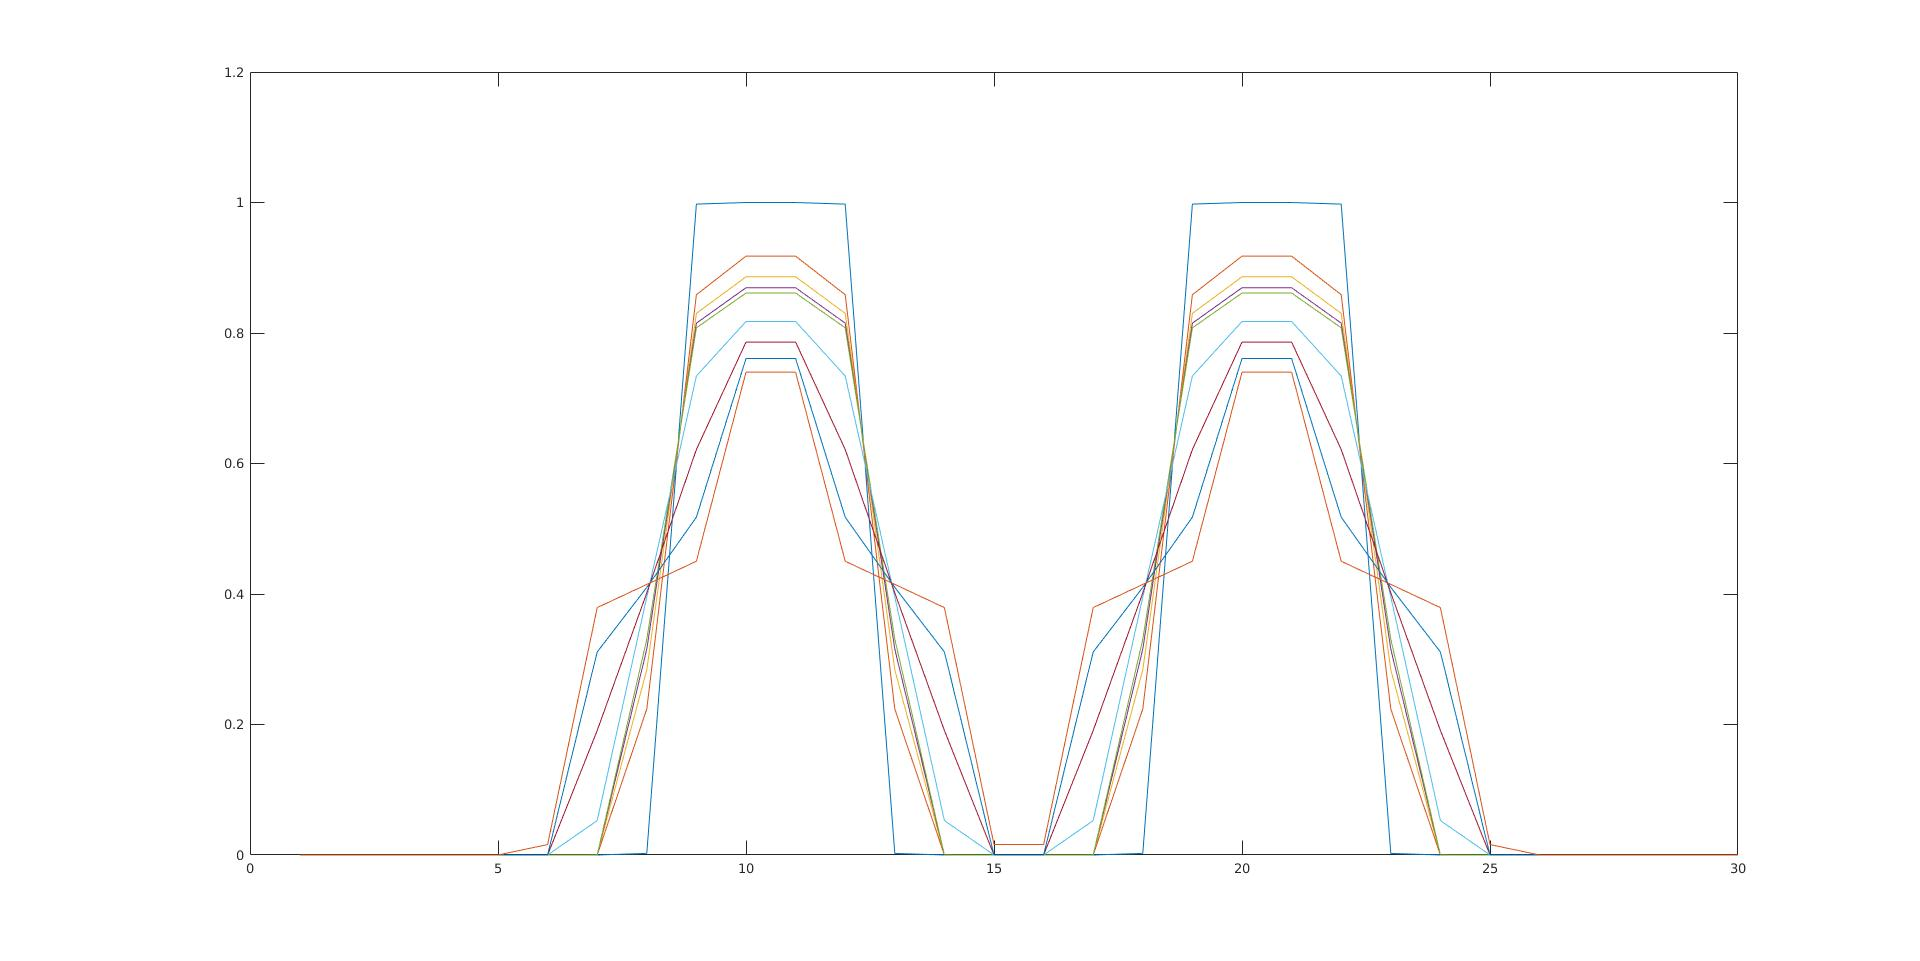
\includegraphics[width=1.1\linewidth]{assets/AlX10}
%   \caption{Результат моделирования старения}
%   \label{img:AlX10}
% \end{figure}

% \section{Моделирование диффузионного размытия в <<открытой системе>> $i\!-\!GaAs/i\!-\!Al_{45}Ga_{55}As$}
% \begin{figure}[h]
%   \centering
%   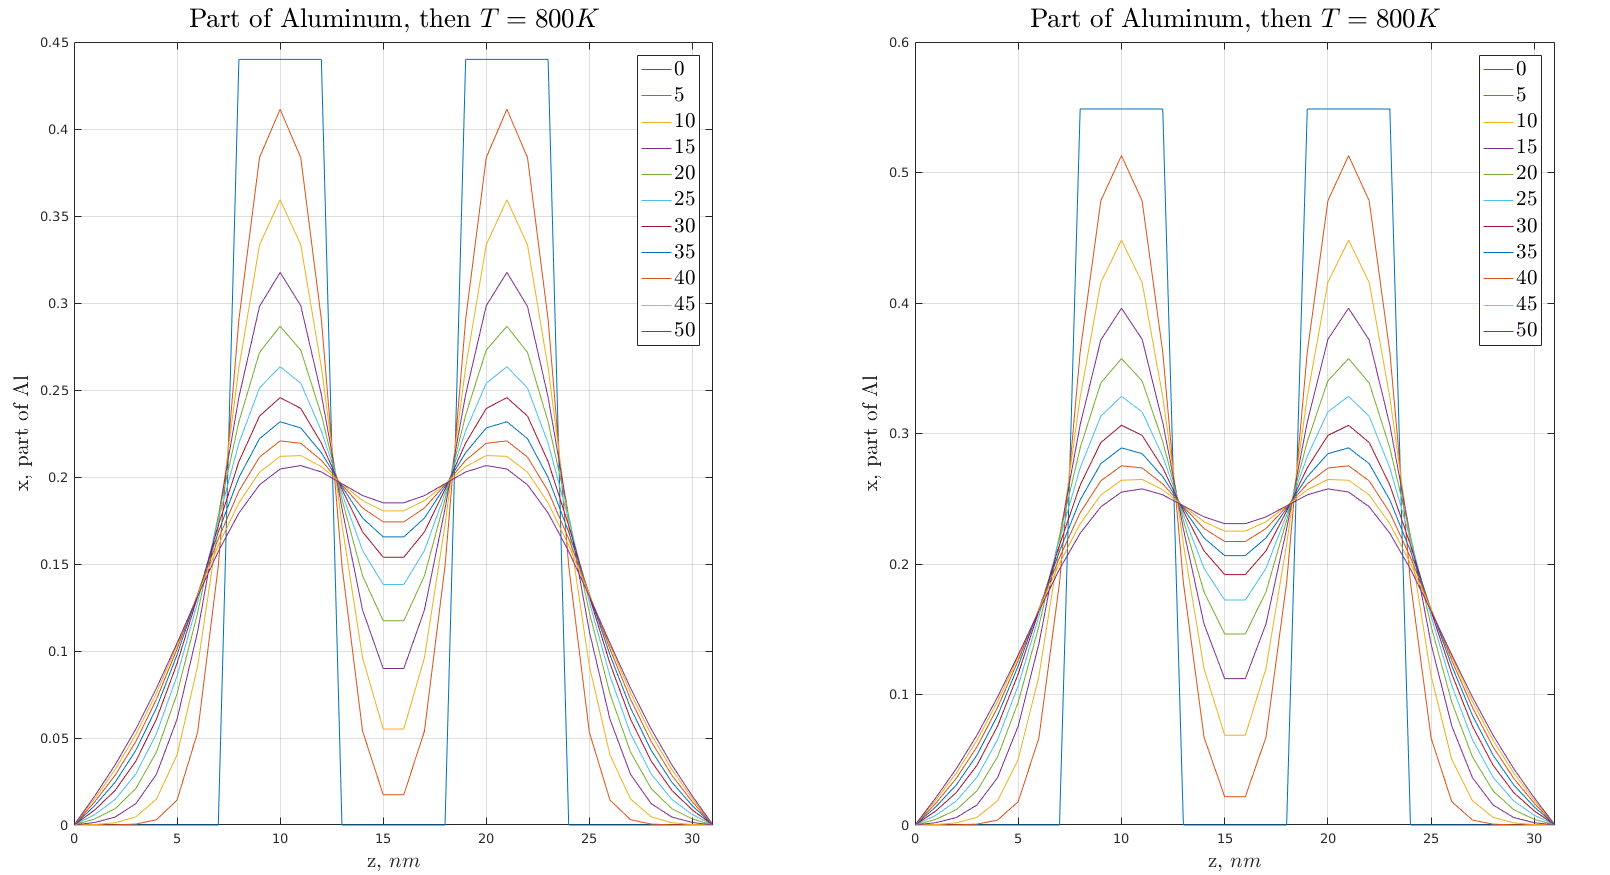
\includegraphics[width=0.9\linewidth]{DOAlGaAs}
%   \caption{Диффузионное размытие}
% \end{figure}

% \begin{figure}[h]
%   \centering
%   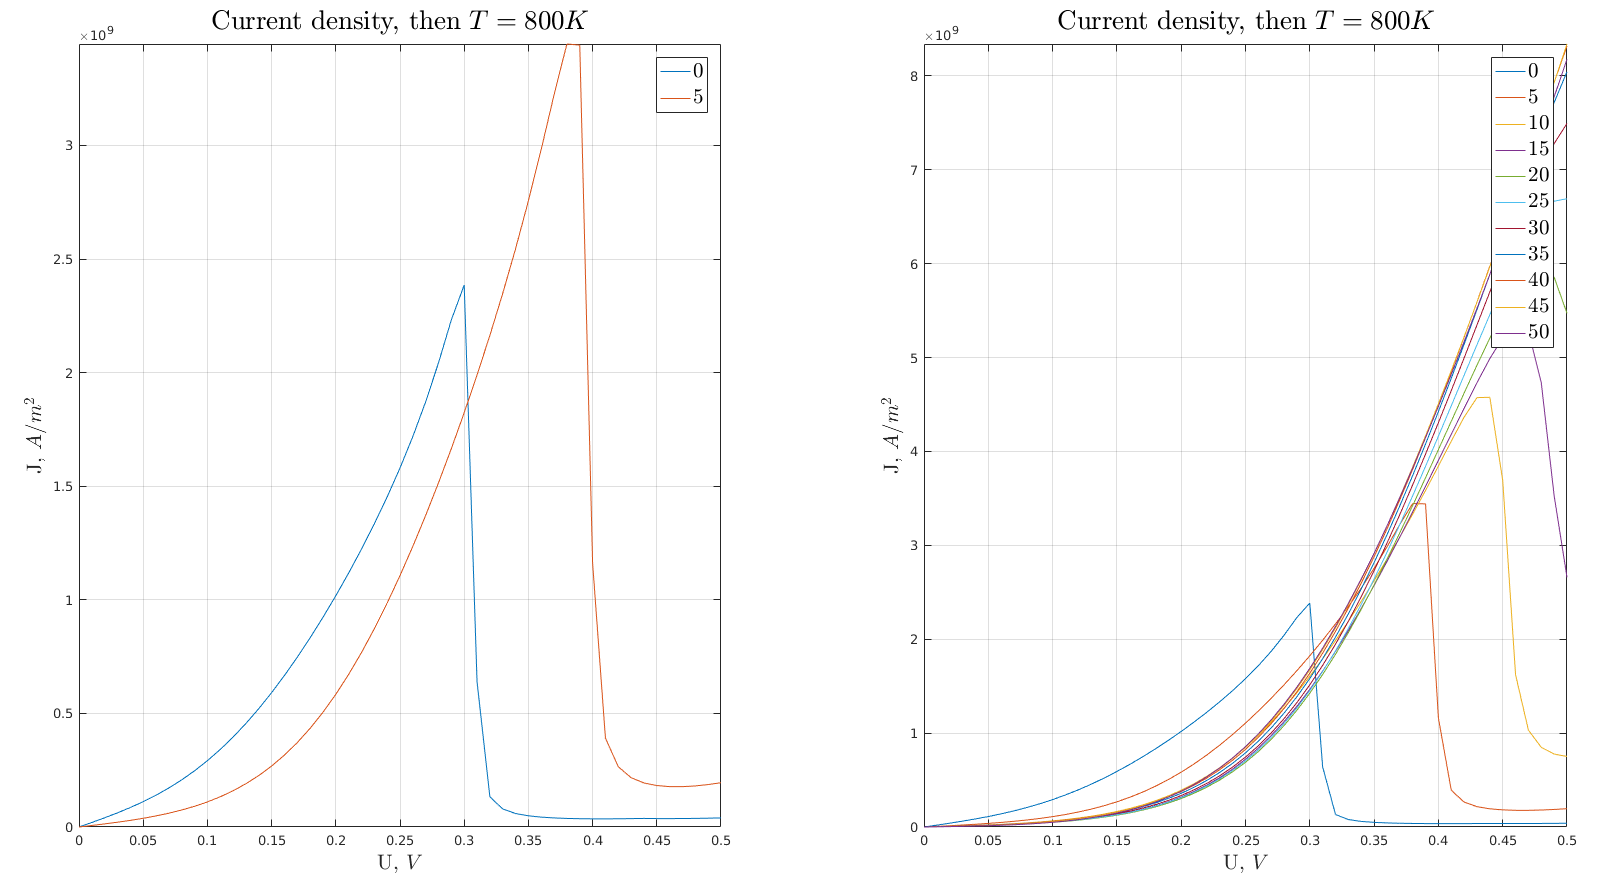
\includegraphics[width=0.9\linewidth]{JDOAlGaAs}
%   \caption{Деградация ВАХ}
% \end{figure}

% \begin{figure}[h]
%   \centering
%   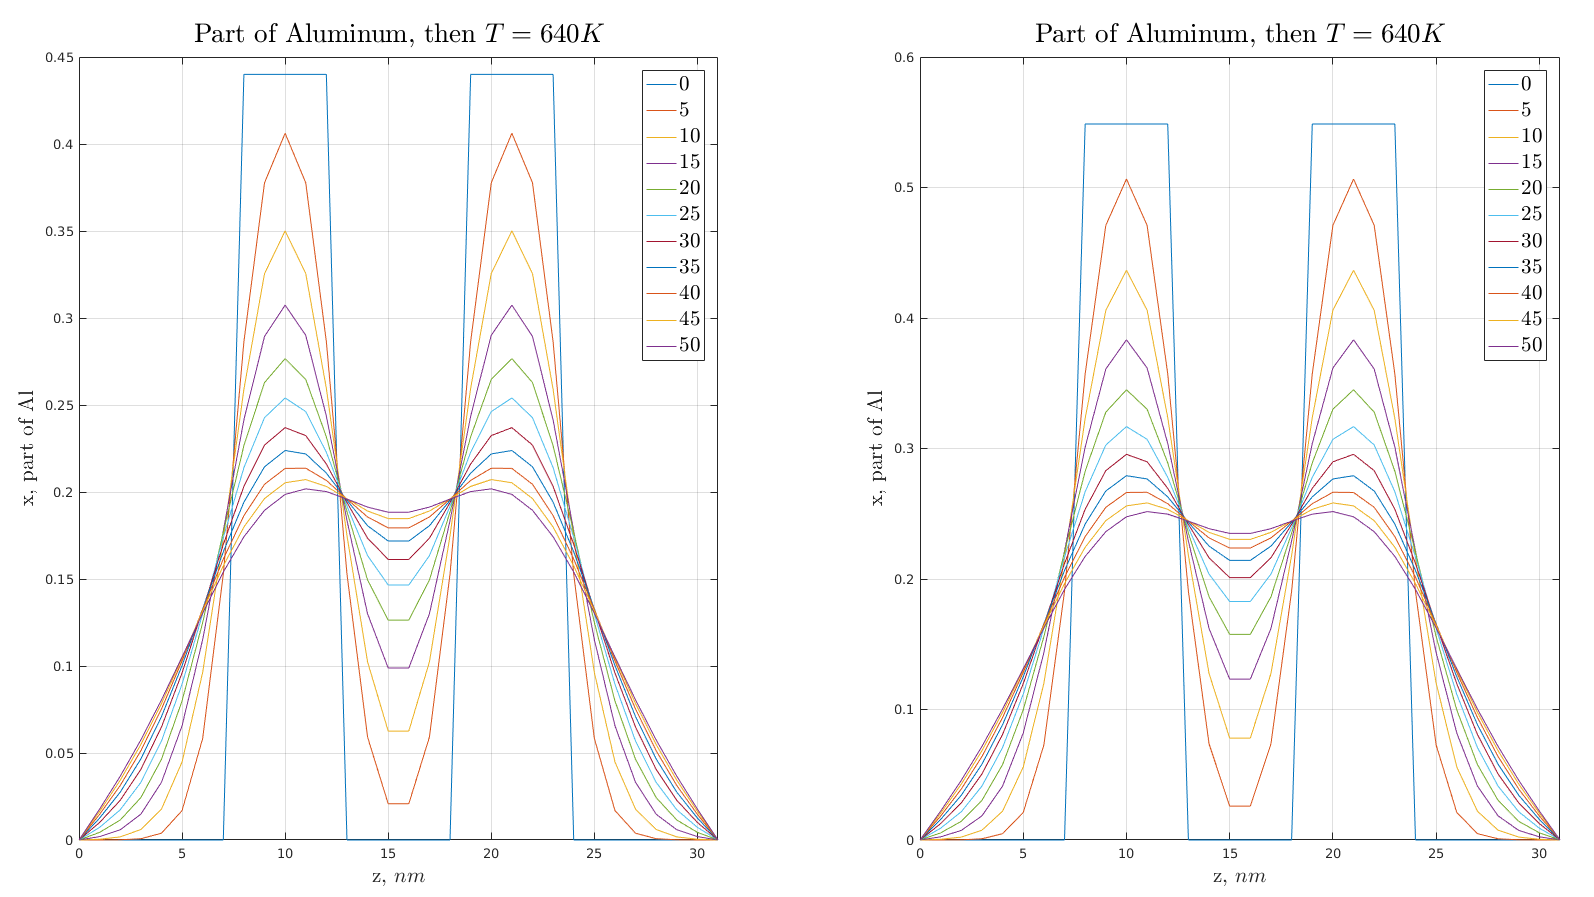
\includegraphics[width=\linewidth]{DOAlGaAsNd}
%   \caption{Диффузионное размытие с учетом примеси, $Nd = 5*10^{15}sm^{-3}$}
% \end{figure}

% \begin{figure}[h]
%   \centering
%   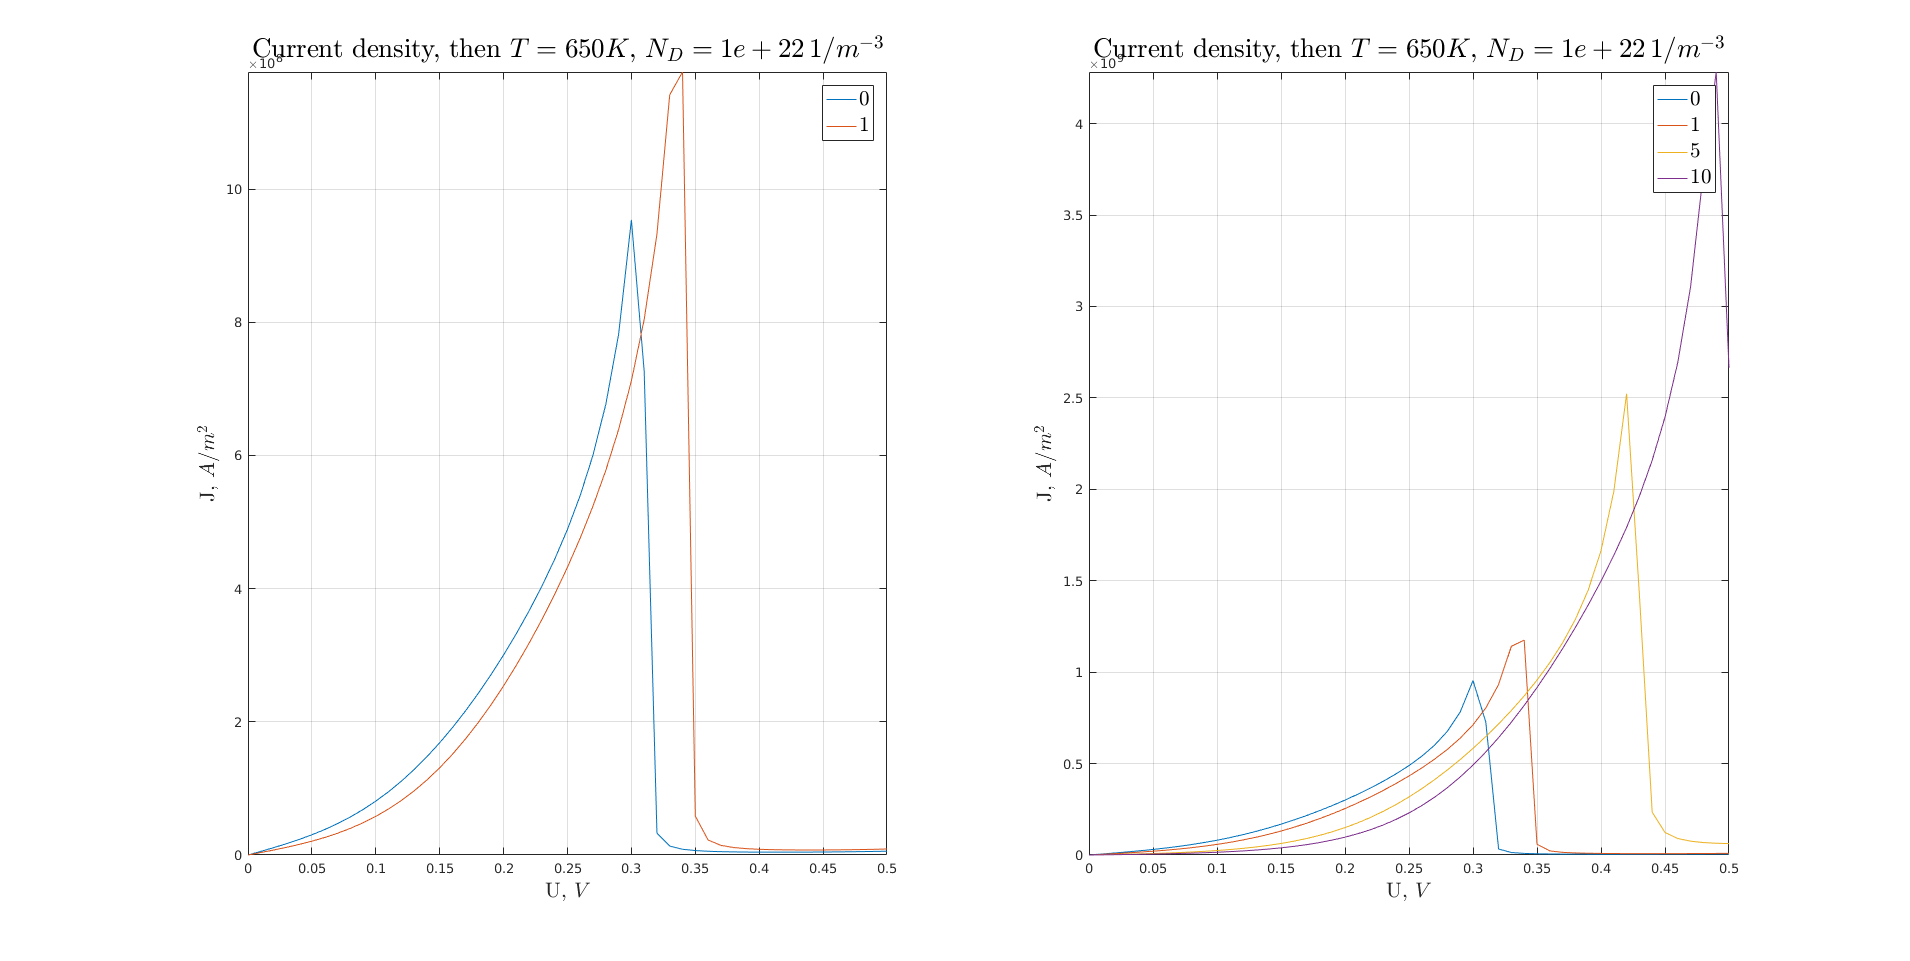
\includegraphics[width=\linewidth]{JDOAlGaAsNd}
%   \caption{Деградация ВАХ с учетом примеси, $Nd = 5*10^{15}sm^{-3}$}
% \end{figure}
\section{Исследование парметров барьеров}

\subsection{Исследование высоты барьеров}
\subsubsection{ВАХ РТГС}
\subsubsection{Прозрачность РТГС}

\subsection{Исследование ширины барьеров}
\subsubsection{ВАХ РТГС}
\subsubsection{Прозрачность РТГС}
	\section{Исследование параметров спейсеров}
Спейсер предназначен для отделения высоколегированной области вырожденного полупроводника от активной. Диффундируя донорная примесь изменяла бы зонную структуру активной (квантовой) области. Так же спейсер препятствует накоплению заряда вблизи барьеров, что влияет на пиковое напряжение и ток.
\subsection{Исследование влияния размеров спейсера}
Рассмотрим спейсеры <<a>>: 
\begin{itemize}
	\item 3 монослоя;
	\item 7 монослоя;
	\item 10 монослоя;
	\item 15 монослоя.
\end{itemize}
\subsubsection{Прозрачность РТГС}

\begin{figure}[h]
	\centering
	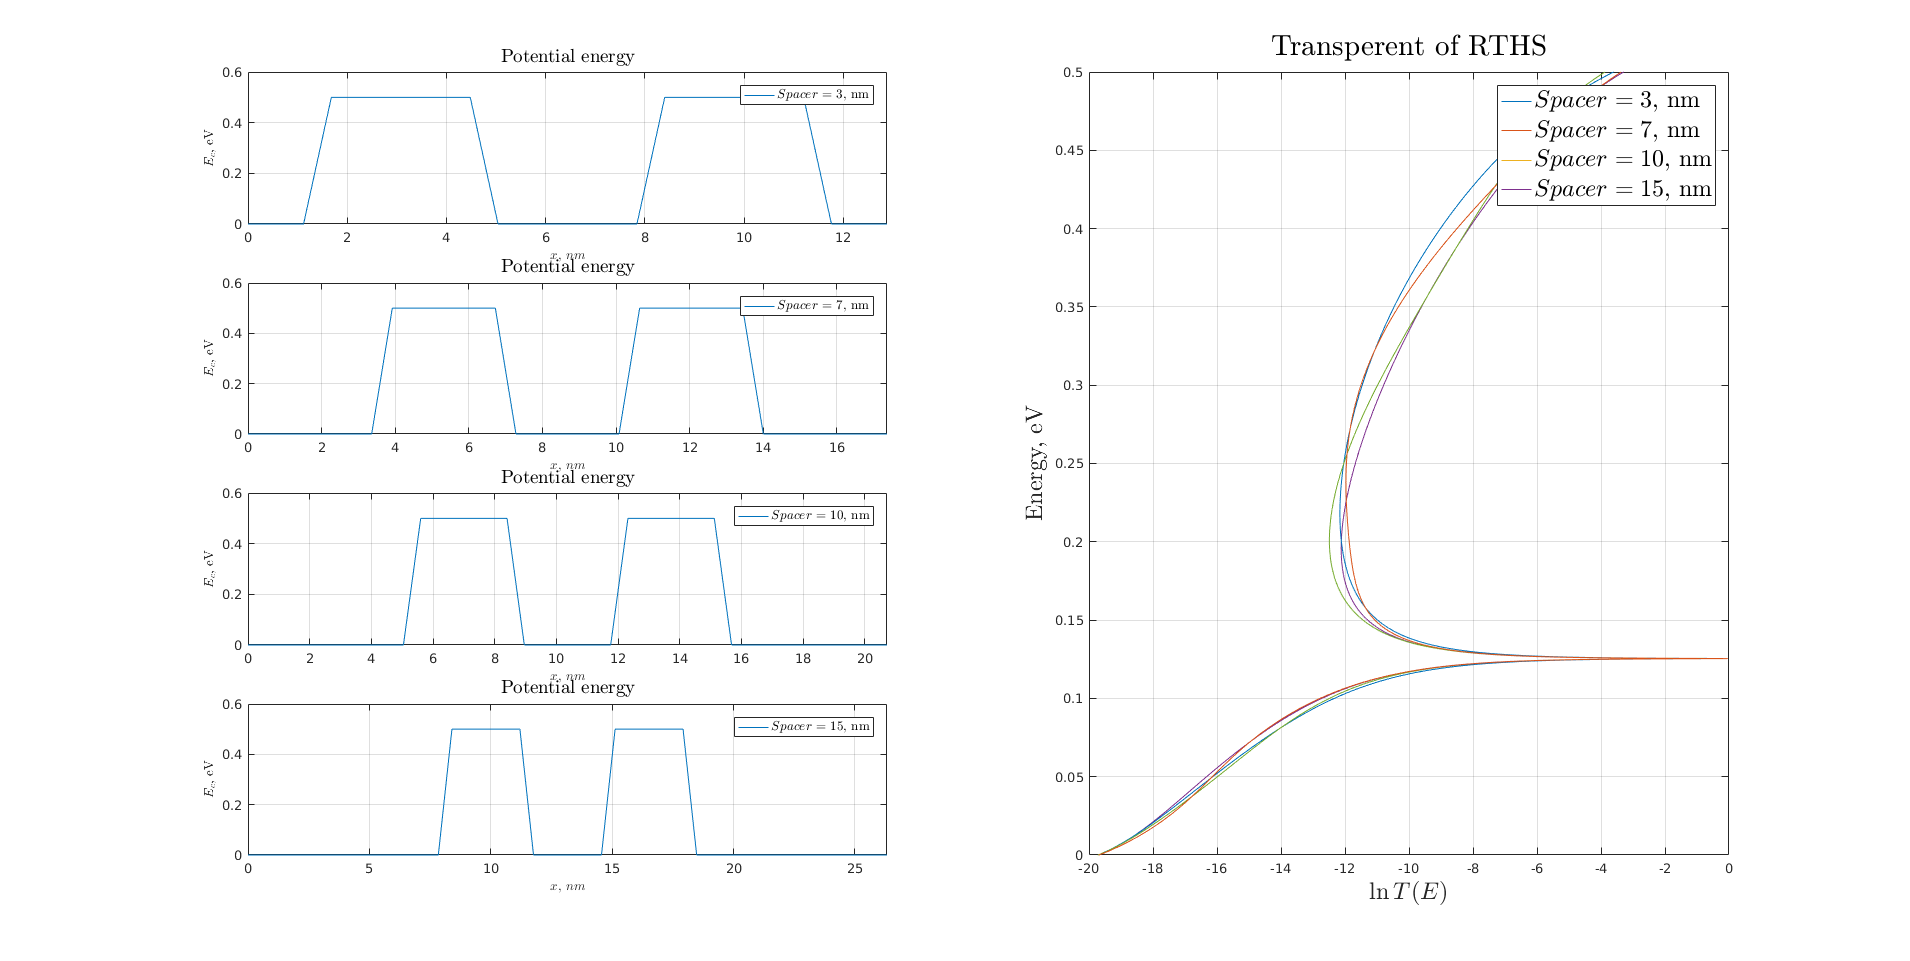
\includegraphics[width=\linewidth]{qslt.png}
	\caption{Прозрачность РТГС при различной ширине спейсеров}
	\label{fig:qslt}
\end{figure}

Прозрачность гетероструктуры изменяется незначительно.

\subsubsection{ВАХ РТГС}
Увеличение размеров спейсера ведет к незначительному (порядок не изменяется), а пиковое напряжение не смещается.

\begin{figure}[h!]
	\centering
	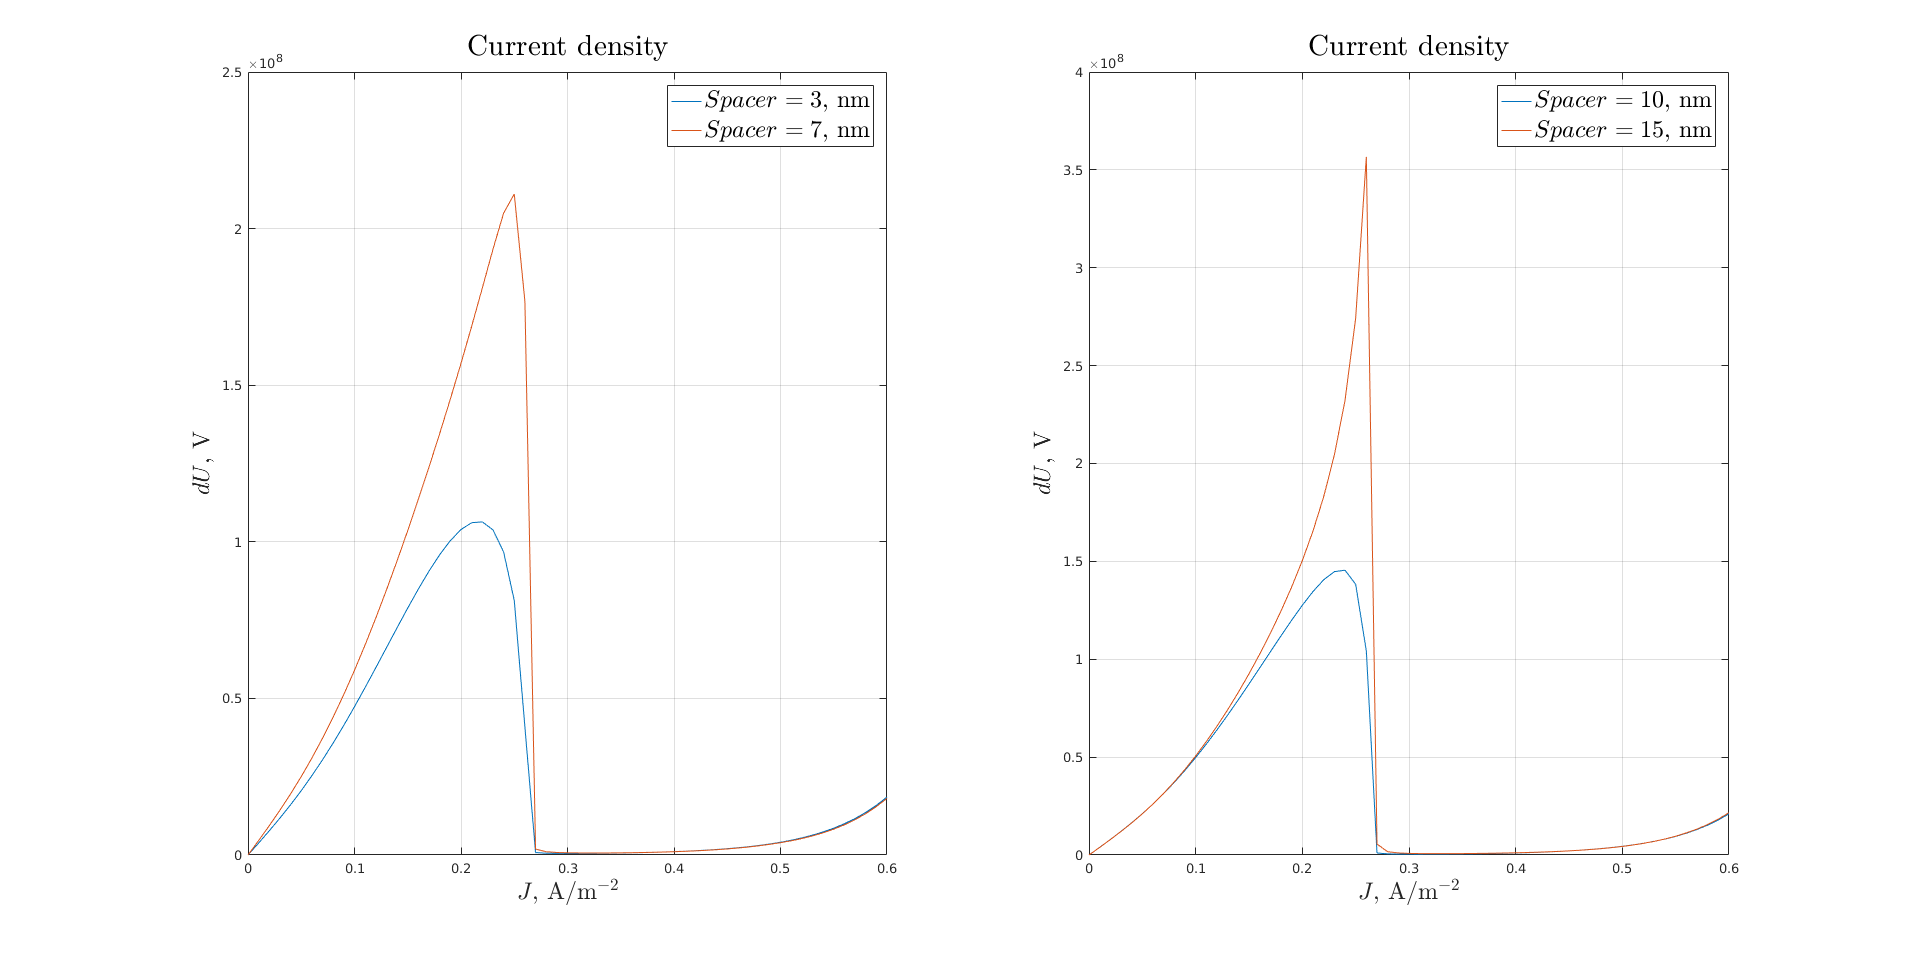
\includegraphics[width=0.9\linewidth]{qslj.png}
	\caption{ВАХ РТГС при различной ширине спейсеров}
	\label{fig:qslj}
\end{figure}


\subsubsection{Учет перераспределения зарядов}
Величина спейсера влияет на накопление заряда вблизи барьеров. Данный эффект сдвигает пиковое напряжение и увеличивает его.

\begin{figure}[h!]
	\centering
	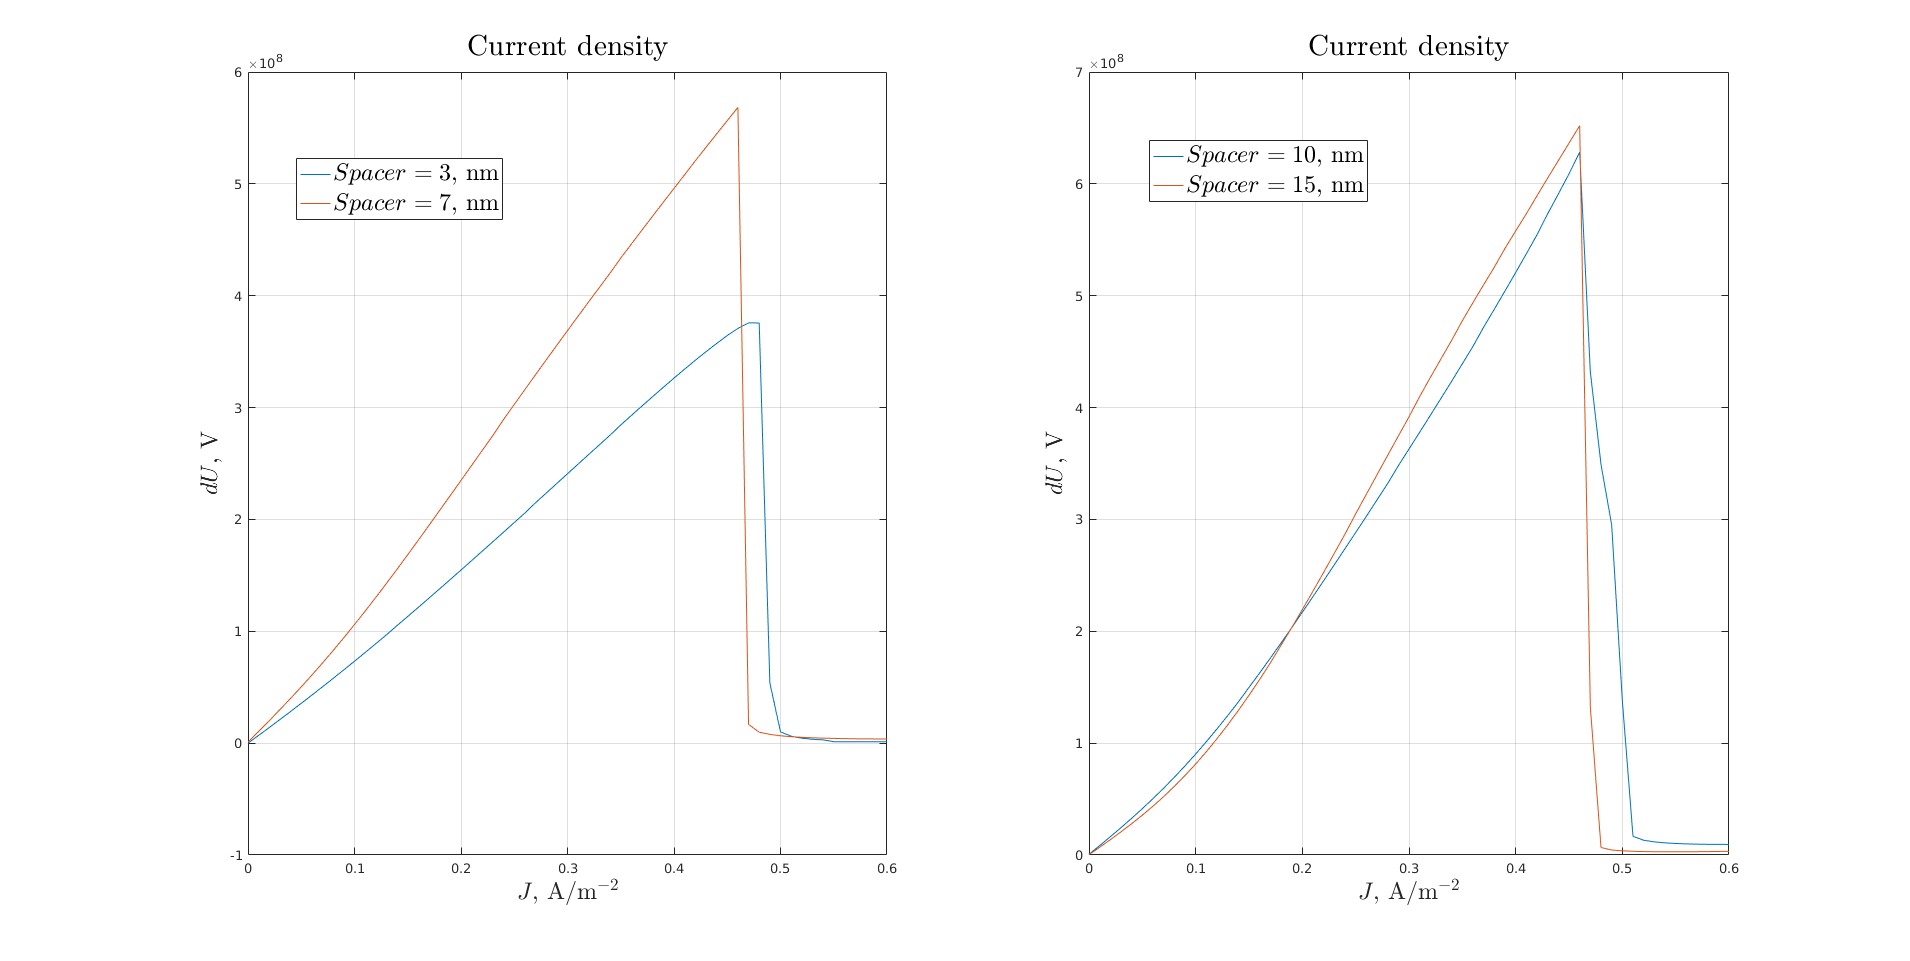
\includegraphics[width=0.9\linewidth]{qslqj.png}
	\caption{ВАХ РТГС при различной ширине спейсеров с учетом перераспределения заряда}
	\label{fig:qslqj}
\end{figure}

\subsection{Вывод}
Из полученных зависимостей видно, что размеры спейсера с учетом перераспределения заряда влияют на ВАХ РТГС при размера менее, чем несколько монослоев. При больших размерах ток через РТГС уменьшается незначительно, так же, как и пиковое напряжение.

\backmatter
% \Conclusion
Сокращение сложности схемы, точности элементарной базы и сокращения элементарной базы не попадают в рамку разумного, так как требуют снижения аж до 80\%, что невозможно.

Исходя из полученных результатов можно сделать вывод, что лучшими оказали специальный холодный и горячий типы резервирования. Общий горячий дает слишком большую кратность $ m =75 $, в то время при специальном резервировании  мы можем резервировать даже не все элементы.

При этом снижение интенсивности отказов элементарной базы на порядок значительно влияет на количество элементов, которых нужно резервировать. Количество элементов не дало существенного прироста эффективности резервирования. Время эксплуатации дало так же весомый вклад в купе со снижением интенсивности.
% \bibliographystyle{gost780u}
\bibliography{index}

\appendix

\end{document}
